% Format teze zasnovan je na paketu memoir
% http://tug.ctan.org/macros/latex/contrib/memoir/memman.pdf ili
% http://texdoc.net/texmf-dist/doc/latex/memoir/memman.pdf
% 
% Prilikom zadavanja klase memoir, navedenim opcijama se podešava 
% veličina slova (12pt) i jednostrano štampanje (oneside).
% Ove parametre možete menjati samo ako pravite nezvanične verzije
% mastera za privatnu upotrebu (na primer, u b5 varijanti ima smisla 
% smanjiti 
\documentclass[12pt,oneside]{memoir}

% Paket koji definiše sve specifičnosti mastera Matematičkog fakulteta
\usepackage[latinica]{matfmaster}
%
% Podrazumevano pismo je ćirilica.
%   Ako koristite pdflatex, a ne xetex, sav latinički tekst na srpskom jeziku
%   treba biti okružen sa \lat{...} ili \begin{latinica}...\end{latinica}.
%
% Opicija [latinica]:
%   ako želite da pišete latiniciom, dodajte opciju "latinica" tj.
%   prethodni paket uključite pomoću: \usepackage[latinica]{matfmaster}.
%   Ako koristite pdflatex, a ne xetex, sav ćirilički tekst treba biti
%   okružen sa \cir{...} ili \begin{cirilica}...\end{cirilica}.
%
% Opcija [biblatex]:
%   ako želite da koristite reference na više jezika i umesto paketa
%   bibtex da koristite BibLaTeX/Biber, dodajte opciju "biblatex" tj.
%   prethodni paket uključite pomoću: \usepackage[biblatex]{matfmaster}
%
% Opcija [b5paper]:
%   ako želite da napravite verziju teze u manjem (b5) formatu, navedite
%   opciju "b5paper", tj. prethodni paket uključite pomoću: 
%   \usepackage[b5paper]{matfmaster}. Tada ima smisla razmisliti o promeni
%   veličine slova (izmenom opcije 12pt na 11pt u \documentclass{memoir}).
%
% Naravno, opcije je moguće kombinovati.
% Npr. \usepackage[b5paper,biblatex]{matfmaster}

% Pomoćni paket koji generiše nasumičan tekst u kojem se javljaju sva slova
% azbuke (nema potrebe koristiti ovo u pravim disertacijama)
\usepackage{pangrami}

% Paket koji obezbeđuje ispravni prikaz ćiriličkih italik slova kada
% se koristi pdflatex. Zakomentarisati ako na sistemu koji koristite ovaj
% paket nije dostupan ili ako ne radi ispravno.
\usepackage{cmsrb}

% Ostali paketi koji se koriste u dokumentu
\usepackage{listings} 

\renewcommand{\lstlistingname}{Primer}


\lstdefinelanguage{JavaScript}{
  morekeywords=[1]{break, continue, delete, else, for, function, if, in,
    new, return, this, typeof, var, void, while, with},
  % Literals, primitive types, and reference types.
  morekeywords=[2]{false, null, true, boolean, number, undefined,
    Array, Boolean, Date, Math, Number, String, Object},
  % Built-ins.
  morekeywords=[3]{eval, parseInt, parseFloat, escape, unescape},
  sensitive,
  morecomment=[s]{/*}{*/},
  morecomment=[l]//,
  morecomment=[s]{/**}{*/}, % JavaDoc style comments
  morestring=[b]',
  morestring=[b]"
}[keywords, comments, strings]

\lstalias[]{ES6}[ECMAScript2015]{JavaScript}

\lstdefinelanguage[ECMAScript2015]{JavaScript}[]{JavaScript}{
  morekeywords=[1]{await, async, case, catch, class, const, default, do,
    enum, export, extends, finally, from, implements, import, instanceof,
    let, static, super, switch, throw, try},
  morestring=[b]` % Interpolation strings.
}

\lstdefinelanguage{docker}{
  keywords={FROM, RUN, COPY, ADD, ENTRYPOINT, CMD,  ENV, ARG, WORKDIR, EXPOSE, LABEL, USER, VOLUME, STOPSIGNAL, ONBUILD, MAINTAINER, HEALTHCHECK},
  keywordstyle=\color{blue}\bfseries,
  identifierstyle=\color{black},
  sensitive=false,
  comment=[l]{\#},
  commentstyle=\color{purple}\ttfamily,
  stringstyle=\color{red}\ttfamily,
  morestring=[b]',
  morestring=[b]"
}

\lstdefinelanguage{docker-compose}{
  keywords={image, environment, ports, container_name, ports, volumes, links},
  keywordstyle=\color{blue}\bfseries,
  identifierstyle=\color{black},
  sensitive=false,
  comment=[l]{\#},
  commentstyle=\color{purple}\ttfamily,
  stringstyle=\color{red}\ttfamily,
  morestring=[b]',
  morestring=[b]"
}
\lstdefinelanguage{docker-compose-2}{
  keywords={version, volumes, services},
  keywordstyle=\color{blue}\bfseries,
  keywords=[2]{image, environment, ports, container_name, ports, links, build},
  keywordstyle=[2]\color{olive}\bfseries,
  identifierstyle=\color{black},
  sensitive=false,
  comment=[l]{\#},
  commentstyle=\color{purple}\ttfamily,
  stringstyle=\color{red}\ttfamily,
  morestring=[b]',
  morestring=[b]"
}

\lstset{basicstyle=\ttfamily,
  showstringspaces=false,
  commentstyle=\color{red},
  keywordstyle=\color{blue},
  inputencoding=utf8,
  extendedchars=true
}

% Requires package: color.
\definecolor{mediumgray}{rgb}{0.3, 0.4, 0.4}
\definecolor{mediumblue}{rgb}{0.0, 0.0, 0.8}
\definecolor{forestgreen}{rgb}{0.13, 0.55, 0.13}
\definecolor{darkviolet}{rgb}{0.58, 0.0, 0.83}
\definecolor{royalblue}{rgb}{0.25, 0.41, 0.88}
\definecolor{crimson}{rgb}{0.86, 0.8, 0.24}

\lstdefinestyle{JSES6Base}{
  backgroundcolor=\color{white},
  basicstyle=\ttfamily,
  breakatwhitespace=false,
  breaklines=false,
  captionpos=b,
  columns=fullflexible,
  commentstyle=\color{mediumgray}\upshape,
  emph={},
  emphstyle=\color{crimson},
  extendedchars=true,  % requires inputenc
  fontadjust=true,
  frame=single,
  identifierstyle=\color{black},
  keepspaces=true,
  keywordstyle=\color{mediumblue},
  keywordstyle={[2]\color{darkviolet}},
  keywordstyle={[3]\color{royalblue}},
  numbers=left,
  numbersep=5pt,
  numberstyle=\tiny\color{black},
  rulecolor=\color{black},
  showlines=true,
  showspaces=false,
  showstringspaces=false,
  showtabs=false,
  stringstyle=\color{forestgreen},
  tabsize=2,
  title=\lstname,
  upquote=true  % requires textcomp
}

\lstdefinestyle{JavaScript}{
  language=JavaScript,
  style=JSES6Base
}
\lstdefinestyle{ES6}{
  language=ES6,
  style=JSES6Base
}

% Datoteka sa literaturom u BibTex tj. BibLaTeX/Biber formatu
\bib{matfmaster}

% Ime kandidata na srpskom jeziku (u odabranom pismu)
\autor{Aleksa Kojadinović}
% Naslov teze na srpskom jeziku (u odabranom pismu)
\naslov{Arhitektura i dizajn veb platforme za upravljanje korisničkim žalbama i zahtevima}
% Godina u kojoj je teza predana komisiji
\godina{2024}
% Ime i afilijacija mentora (u odabranom pismu)
\mentor{Vladimir Filipović}
% Ime i afilijacija prvog člana komisije (u odabranom pismu)
\komisijaA{Saša Malkov}
% Ime i afilijacija drugog člana komisije (u odabranom pismu)
\komisijaB{Aleksandar Kartelj}
% Ime i afilijacija trećeg člana komisije (opciono)
% \komisijaC{}
% Ime i afilijacija četvrtog člana komisije (opciono)
% \komisijaD{}
% Datum odbrane (obrisati ili iskomentarisati narednu liniju ako datum odbrane nije poznat)
\datumodbrane{xx. januar xxxx.}

\setcounter{tocdepth}{3}


% Apstrakt na srpskom jeziku (u odabranom pismu)
\apstr{%
Razvoj veb aplikacija u današnje vreme jedna je od najrasprostranjenijih grana softverskog inženjerstva. Moguće je implementirati veoma kompleksne softverske sisteme kao veb servise. U ovom radu se razmatra i analizira arhitektura kompleksne veb platforme za rešavanje konkretnog poslovnog problema - asinhrone korisničke podrške u vidu kartica. Predloženo rešenje razvijeno je korišćenjem modernih veb tehnologija zasnovanih na Node.js ekosistemu. Rad prikazuje proces dizajna domenskog modela putem ER dijagrama i DDD principa, a zatim i kompletnu implementaciju serverskog i klijentskog dela aplikacije u okruženjima NestJS i Next.js. Pored domenskog dizajna i razvoja, razmatra se i izolacija okruženja koristeći sistem za virtuelizaciju Docker. Rad obuhvata i prikaz implementacije minimalnog analitčkog servisa u jeziku \textit{python} uključujući ETL procese i vizuelizaciju.
}

% Ključne reči na srpskom jeziku (u odabranom pismu)
\kljucnereci{veb, DDD, servisi, API, analitika}

\begin{document}
% ==============================================================================
% Uvodni deo teze
\frontmatter
% ==============================================================================
% Naslovna strana
\naslovna
% Strana sa podacima o mentoru i članovima komisije
\komisija
% Strana sa posvetom (u odabranom pismu)
% Strana sa podacima o disertaciji na srpskom jeziku
\apstrakt
% Sadržaj teze
\tableofcontents*

% ==============================================================================
% Glavni deo teze
\mainmatter
% ==============================================================================

% ------------------------------------------------------------------------------
\chapter{Uvod}

Prilikom razvoja bilo kakvog poslovnog softvera namenjenog za korišćenje od strane velikog broja zaposlenih neke kompanije, u današnje vreme pribegava se implementaciji datog sistema kao jedne kompleksne veb platforme. Razlozi za izbor veba su mnogobrojni, uključujući:

\begin{itemize}
    \item \textbf{Univerzalnost veb pregledača kao platforme na kojoj se izvršava aplikacija.} U kontekstu vizuelnog dela aplikacije, prilikom razvoja tradicionalnih desktop aplikacija potrebno je voditi računa o mogućnosti pokretanja na različitim platformama i arhitekturama, kao i restrikcija pojedinih sistema. Razlike između veb pregledača, iako postoje, jesu umanjene\footnote{I u situacijama kada su značajne postoje alati za njihovo prevazilaženje, kao što je \textit{corejs}.}. 
    \item \textbf{Lakše ažuriranje aplikacije.} Ažuriranje desktop aplikacije često zahteva korisničku akciju u vidu nekakve instalacije, tako da implementacija ovakvog sistema nije trivijalna. U slučaju veba ovo je značajno olakšano zbog same prirode klijent-server ahitekture.
    \item \textbf{Integracije sa eksternim servisima.} Uveliko ustanovljeni veb standardi, kao što je REST API\footnote{O REST API-u će biti reči u sekciji \ref{sec:restapi}.} doveli su do olakšane međusobne integracije veb platformi.
\end{itemize}

Veb je od svog originalnog oblika, koji se zasnivao na prikazivanju i povezivanju statičkih HTML stranica, evoluirao do kompleksne platforme za razvoj softvera. Iz tog razloga vremenom se javljala potreba za formalizovanjem principa razvoja softvera za veb, baš kao i za tradicionalne aplikacije \cite{web_evolution}. Za ove potrebe nastali su mnogi standardi i okviri za uspešan razvoj veb aplikacija, koji se vremenom pokazuju kao dobre prakse uprkos konstantnom menjaju konkretnih tehnologija i trendova.

Ovaj rad predstaviće razvoj kompleksne veb platforme za upravljanje korisničkim žalbama i zahtevima. Pod kompleksnošću platforme primarno se podrazumeva tehnička kompleksnost - mogućnosti sistema iz ugla korisnika su ograničene, ali način na koji je sistem dizajniran omogućava njegovo lako proširenje. Iako se dobri standardi i prakse razvoja veb aplikacija obično vezuju za tradicionalne platforme, cilj ovog rada jeste da predstavi njihovu upotrebljivost i u modernim bibliotekama i okruženjima.

Poglavlje 2 najpre će prikazati sistem STS iz ugla korisnika, kako bi bila jasna problematika realnog sveta koja se rešava, dok se naredni deo bavi projektovanjem sistema putem modela entiteta i odnosa. 

Treće poglavlje bavi se serverskim delom aplikacije, odnosno bekendom, primenom domenskog dizajna i pregledom svakog od slojeva serverske aplikacije.

U poglavlju 4 fokus se prebacuje na klijentski deo aplikacije, gde se osim prikaza rada aplikacije daje i kratak istorijat primene jezika Javascript, kao i na neke druge aspekte razvoja klijentskih aplikacija.

Naredno poglavlje prikazuje implementaciju minimalnog sistema za analitiku, uz propratne ETL procese i vizuelizaciju.

Pretposlednje poglavlje uvodi nas u postavku infrastrukture za razvoj, koncept veb servera i proksija, kao i kratak prikaz sistema Docker, kao neizostavnog alata za moderan veb razvoj.

Poglavlje 7 daje zaključna razmatranja.

\chapter{Sistem STS}
Svaki biznis koji pruža neku vrstu usluge korisnicima neizostavno mora imati korisničku podršku u nekom obliku. Pre razvoja veb tehnologija telefonski sistemi bili su jedini način direktne podrške koju korisnik može da dobije. Razvoj i pristupčanost veba doveli su do evolucije sofisticiranih onlajn proizvoda koji rešavaju problem korisničke podrške, kako putem pisanih rasprava u vidu kartica, tako i putem tradicionalnih telefonskih linija uz određenu integraciju\footnote{\href{http://zendesk.com}{Zendesk}, \href{https://www.8x8.com/}{8x8}, \href{https://www.atlassian.com/software/jira/service-management}{Jira Service Management}.}.


\section{Sistem STS iz ugla korisnika}

Sistem STS\footnote{Skraćeno od eng. Simple Ticket Service, jednostavan servis za kartice.}, razvijan za potrebe ovog rada, obuhvata osnovnu funkcionalnost za pružanje podrške u vidu kartica. Kartica predstavlja jednu tekstualnu korisničku žalbu ili zahtev, na kojoj se može pokrenuti diskusija, a sve sa ciljem asinhronog\footnote{Pod asinhronošću podrazumeva se suprotnost u odnosu na telefonski sistem u kom korisnik i agent podrške vode komunikaciju u realnom vremenu.} razrešenja korisničkog problema. Glavni akteri sistema su:

\begin{itemize}
    \item \textbf{Klijenti} - koji mogu postavljati kartice u cilju dobijanja podrške.
    \item \textbf{Agenti} - koji su zaduženi da odgovaraju na kartice, upravljaju njihovim statusima i rešavaju probleme.
    \item \textbf{Administratori} - zaduženi za podešavanje sistema, dodeljivanje uloga korisnicima, zabranu pristupa korisnicima, ili uopšteno bavljenje kompleksnim problemima.
\end{itemize}

\subsection{Osnovne funkcionalnosti, prikaz kartice, statusi}

Osnovni pojam sistema, kao što je rečeno, jeste kartica. Na slici se vidi primer zaglavlja jedne kartice. Sastoji se primarno iz naslova i opisa, dok se mogu videti imena klijenta i trenutno zaduženog agenta.

\begin{figure}[h]
  \centering
  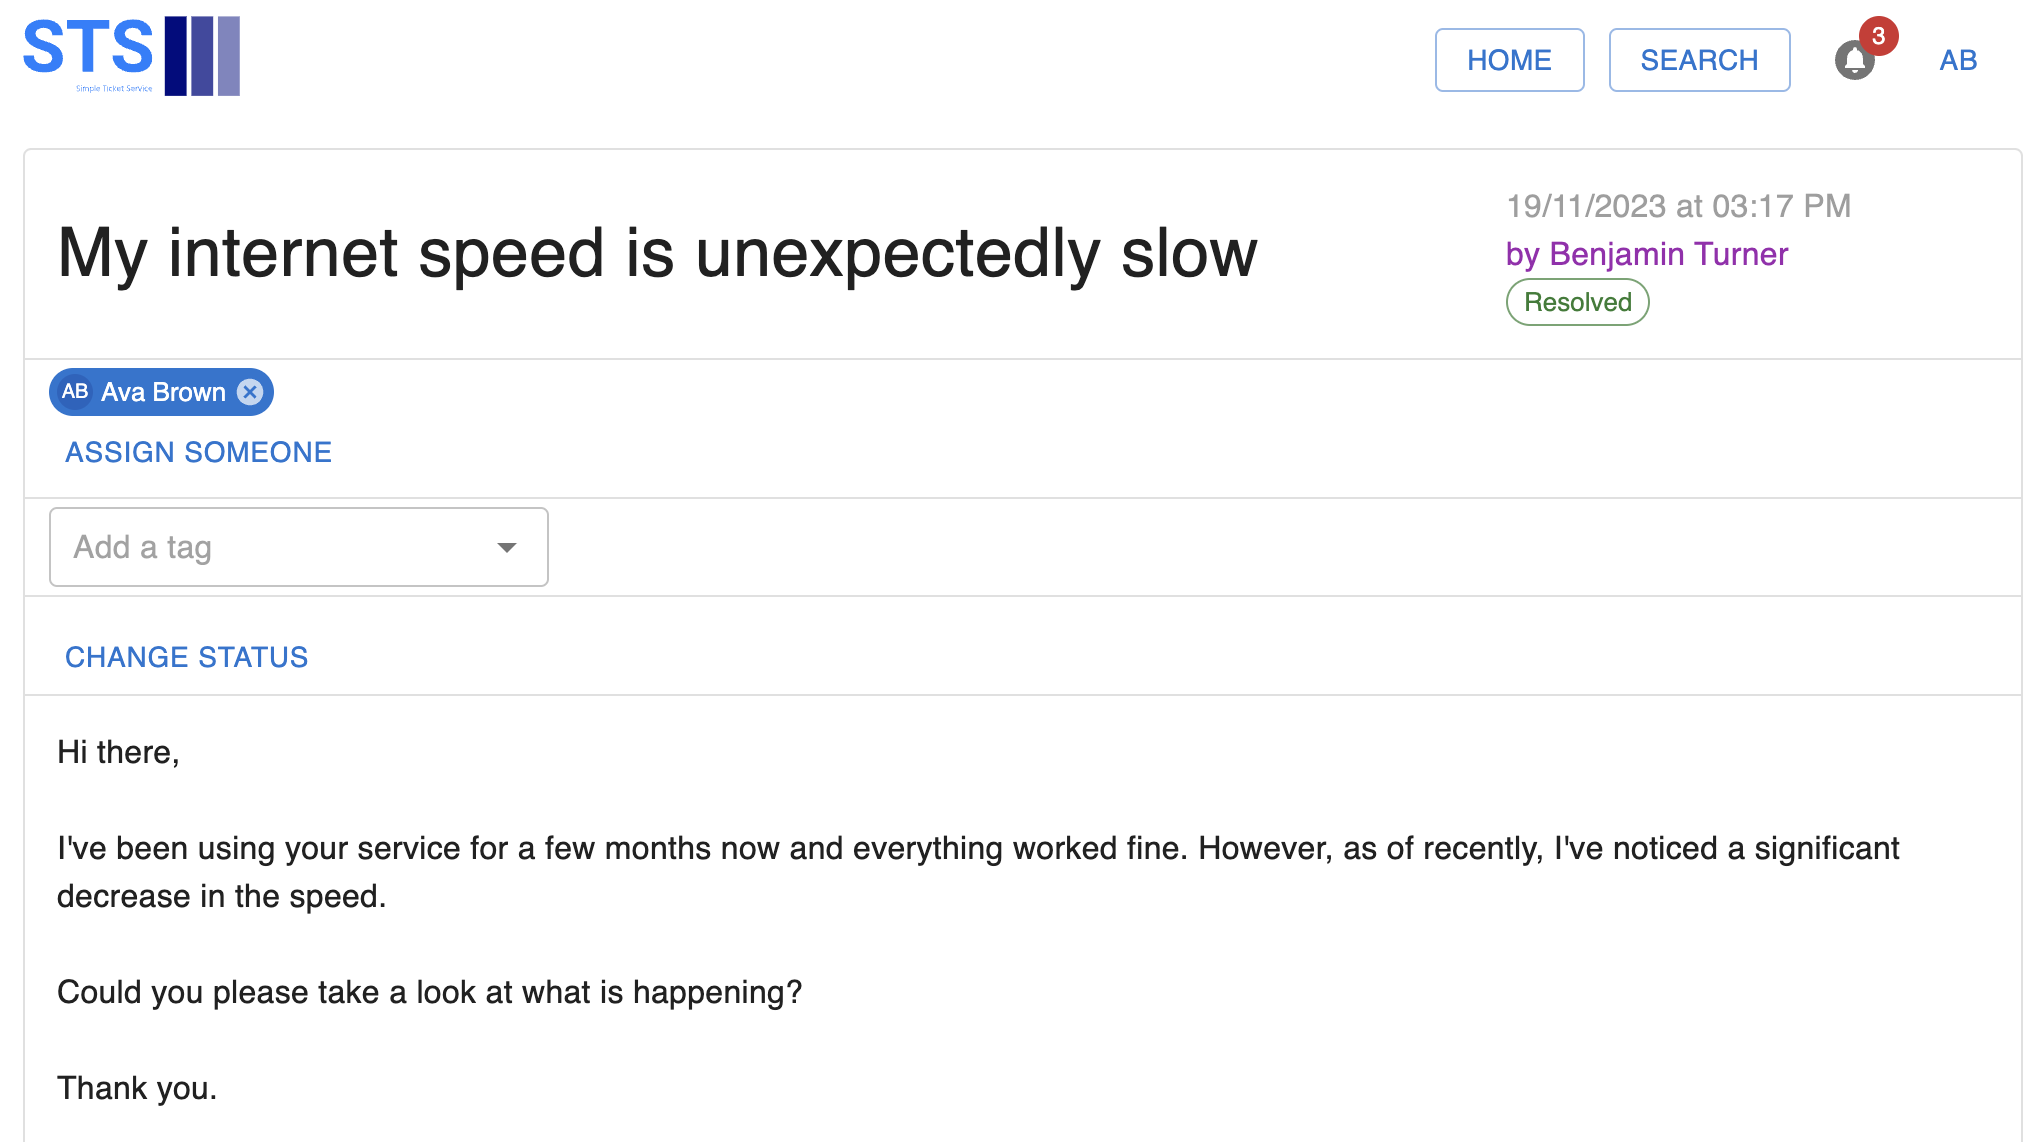
\includegraphics[width=1\textwidth]{docs/images/ch_1/ticket-title.png} 
  \caption{Primer kartice.}
\end{figure}

Kartica može prolaziti kroz više statusa. Promene tih statusa vidljive su kako agentima tako i korisnicima.

\begin{figure}[h]
  \centering
  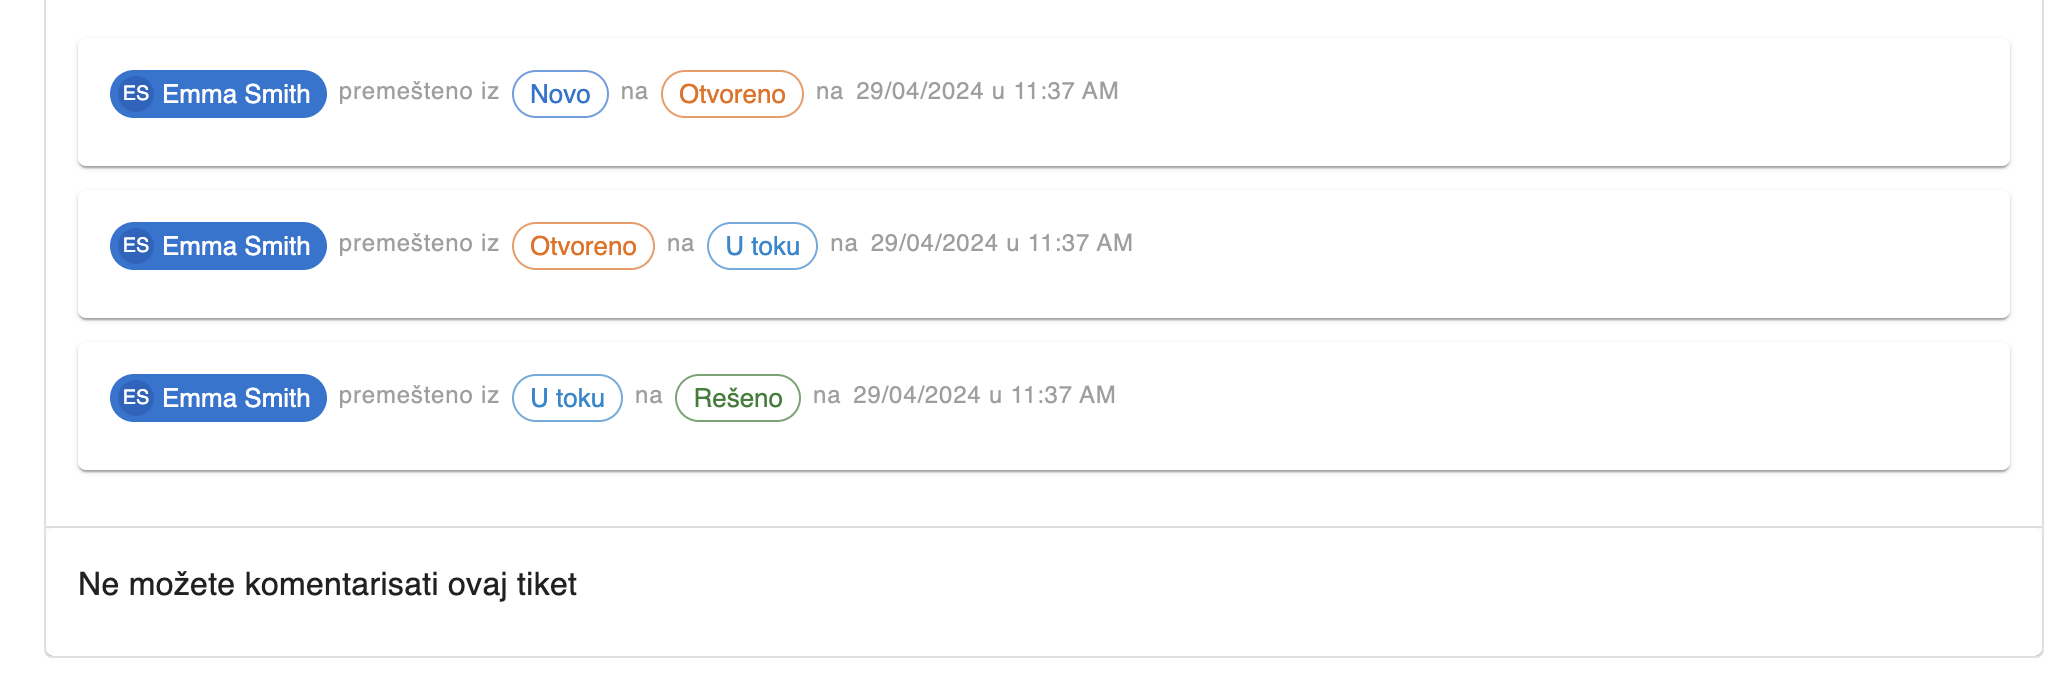
\includegraphics[width=1\textwidth]{docs/images/ch_1/ticket-statuses.png} 
  \caption{Promene statusa.}
\end{figure}

\subsection{Sistem oznaka, konfigurabilnost}
\label{sec:tagsystem}

Često postoji potreba klasifikacije kartica po raznim kriterijumima - departman unutar firme koji se bavi karticom, hitnost, prioritetnost i slično. Kako bi se postigla maksimalna fleksibilnost uveden je sistem oznaka (eng. tags). Oznaka se može nakačiti na datu karticu i može dati brzu informaciju o nekim njegovim aspektima. Ovaj sistem u potpunosti je konfigurabilan od strane korisnika (u ovom slučaju administratora), tako da nije potrebna intervencija programera prilikom dodavanja novih ili promene postojećih oznaka.

Na sledećoj slici vidi se kako izgleda kartica označena oznakama histnosti i odeljenja.

\begin{figure}[h]
  \centering
  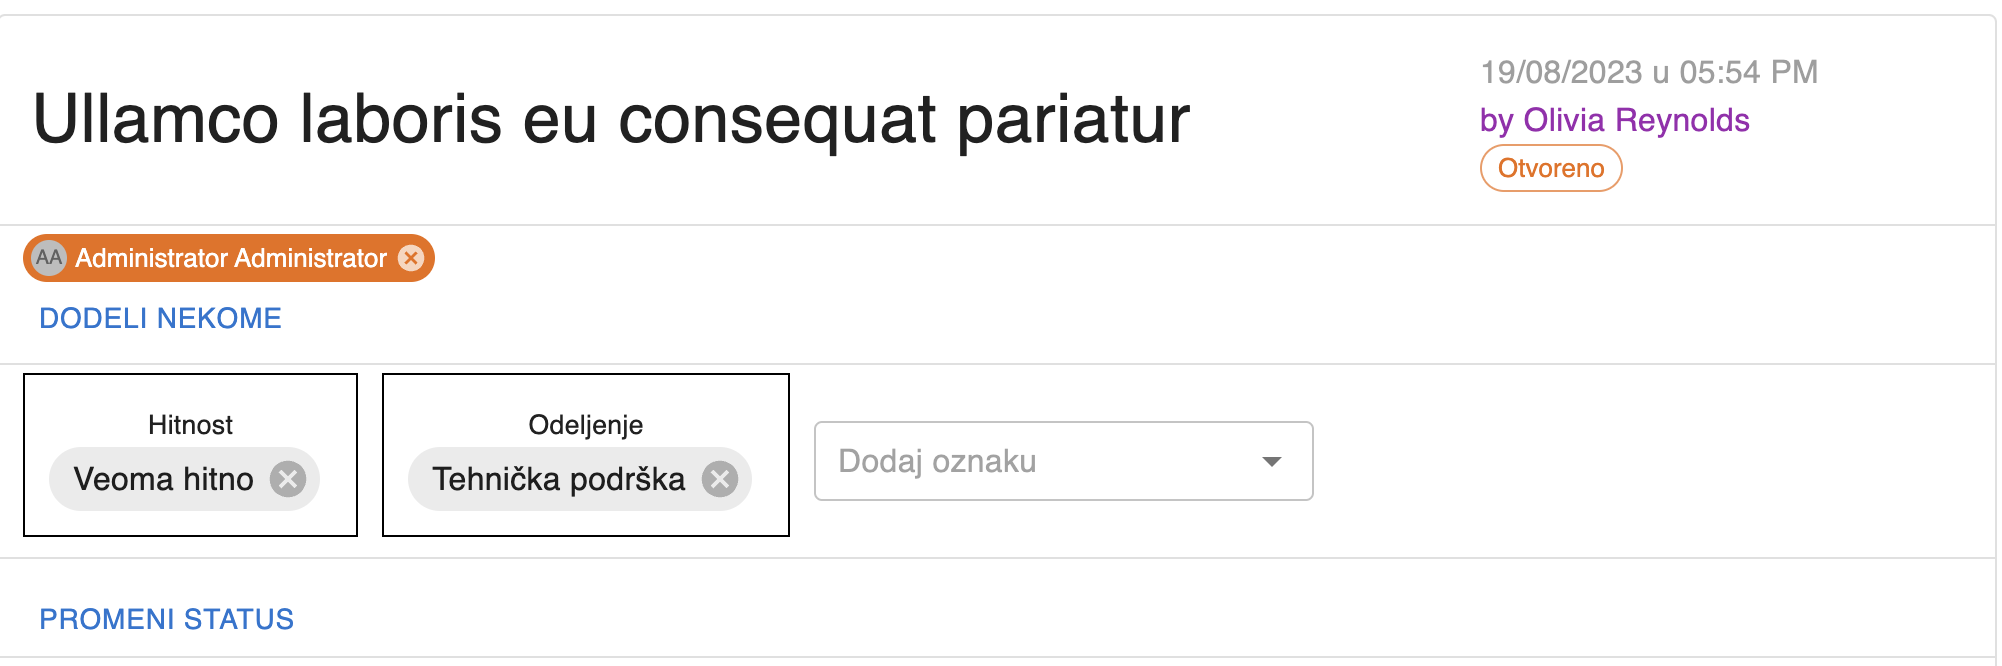
\includegraphics[width=1\textwidth]{docs/images/ch_1/tagged-ticket.png} 
  \caption{Kartica sa oznakama hitnosti i odeljenje.}
\end{figure}

Sledeće dve slike prikazuju kontrolnu tablu na kojoj administatori mogu upravljati oznakama. Primetna je dodatna fleksibilnost u sistemu kojom se može konfigurisati koji tip korisnika ima pravo da vidi, dodaje i uklanja koju oznaku. Takođe može se primetiti da sistem podržava višejezičnost, tako što se imena i opisi mogu podešavati i na srpskom i na engleskom jeziku. O jezicima i sistemu internacionalizacije biće više reči u sekciji \ref{sec:intl}.

\begin{figure}[h]
  \centering
  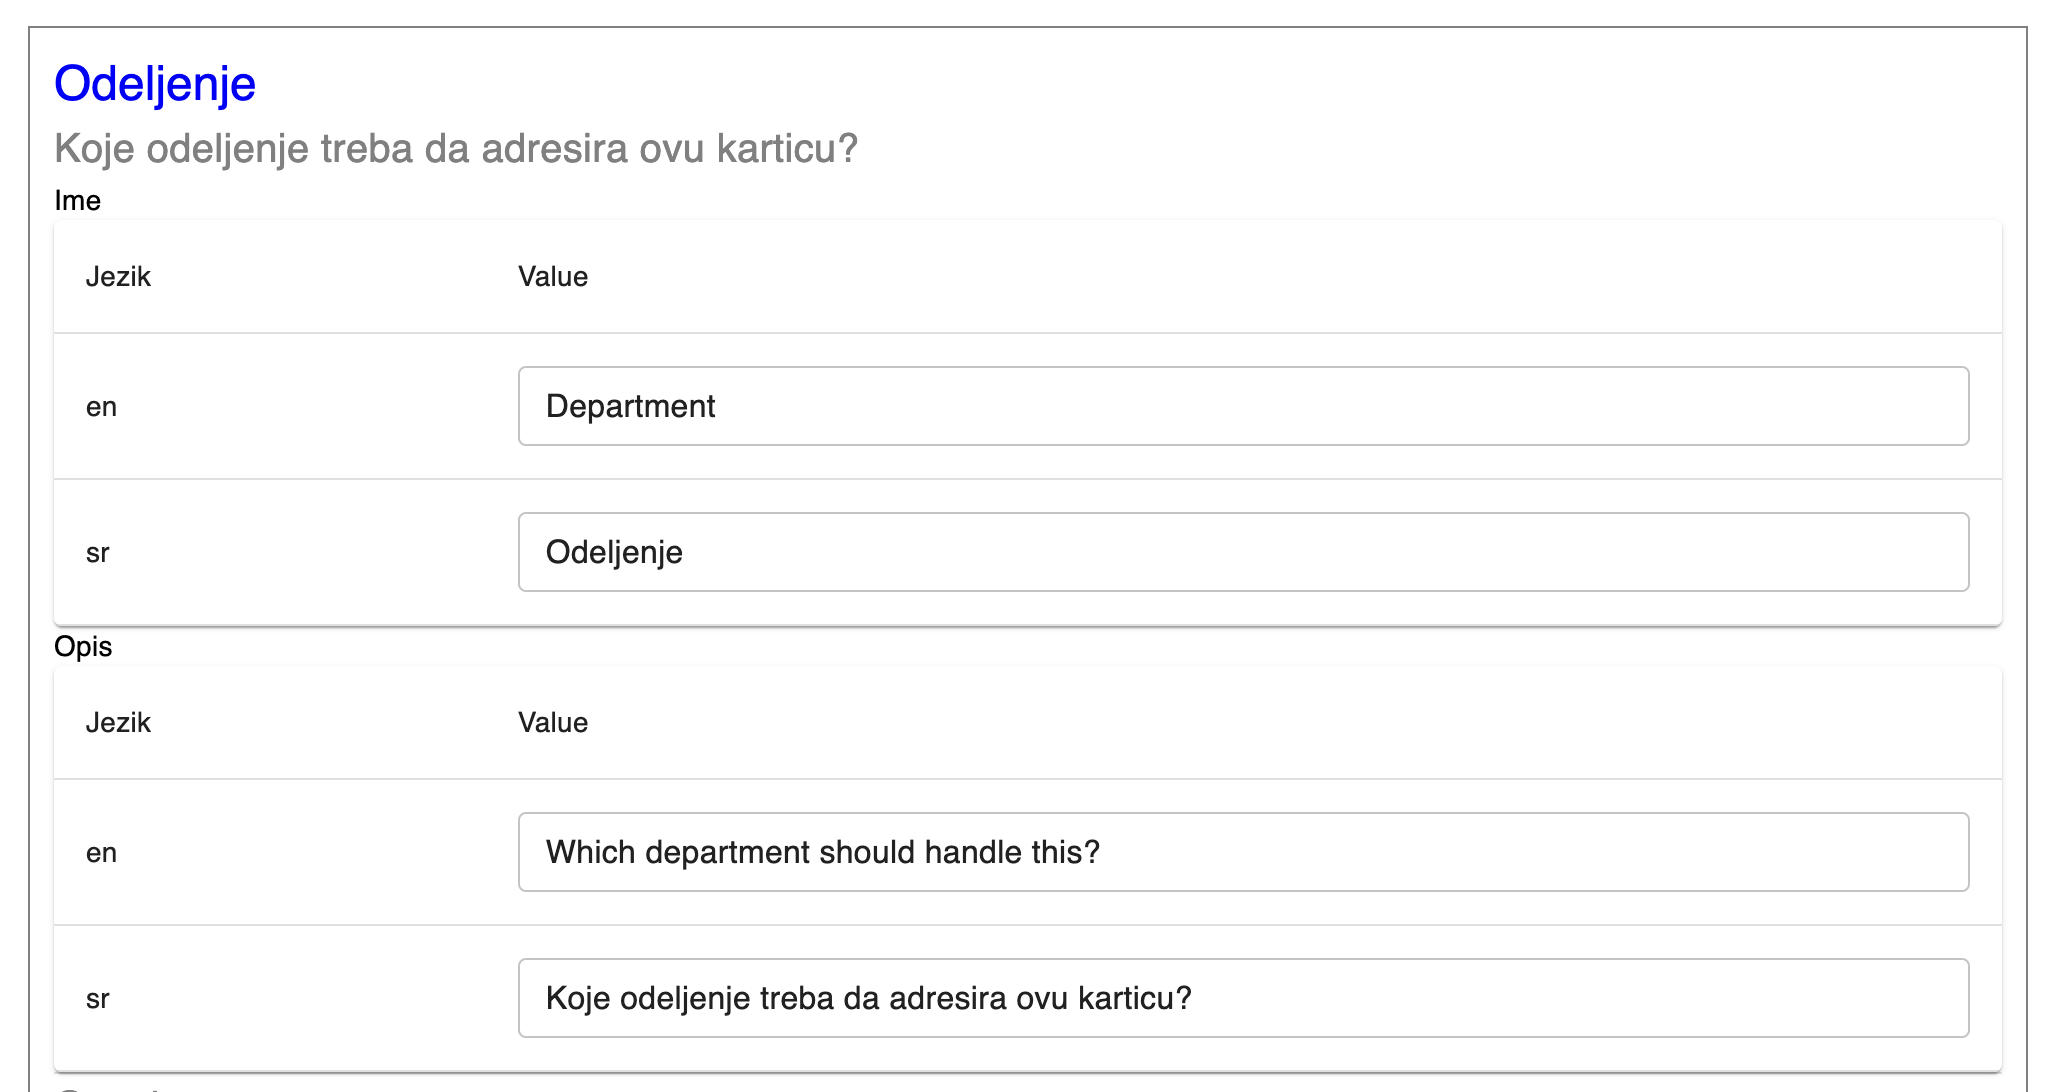
\includegraphics[width=1\textwidth]{docs/images/ch_1/tag-mgmt-head.png} 
  \caption{Kreiranje oznake, višejezička imena.}
\end{figure}

\begin{figure}[h]
  \centering
  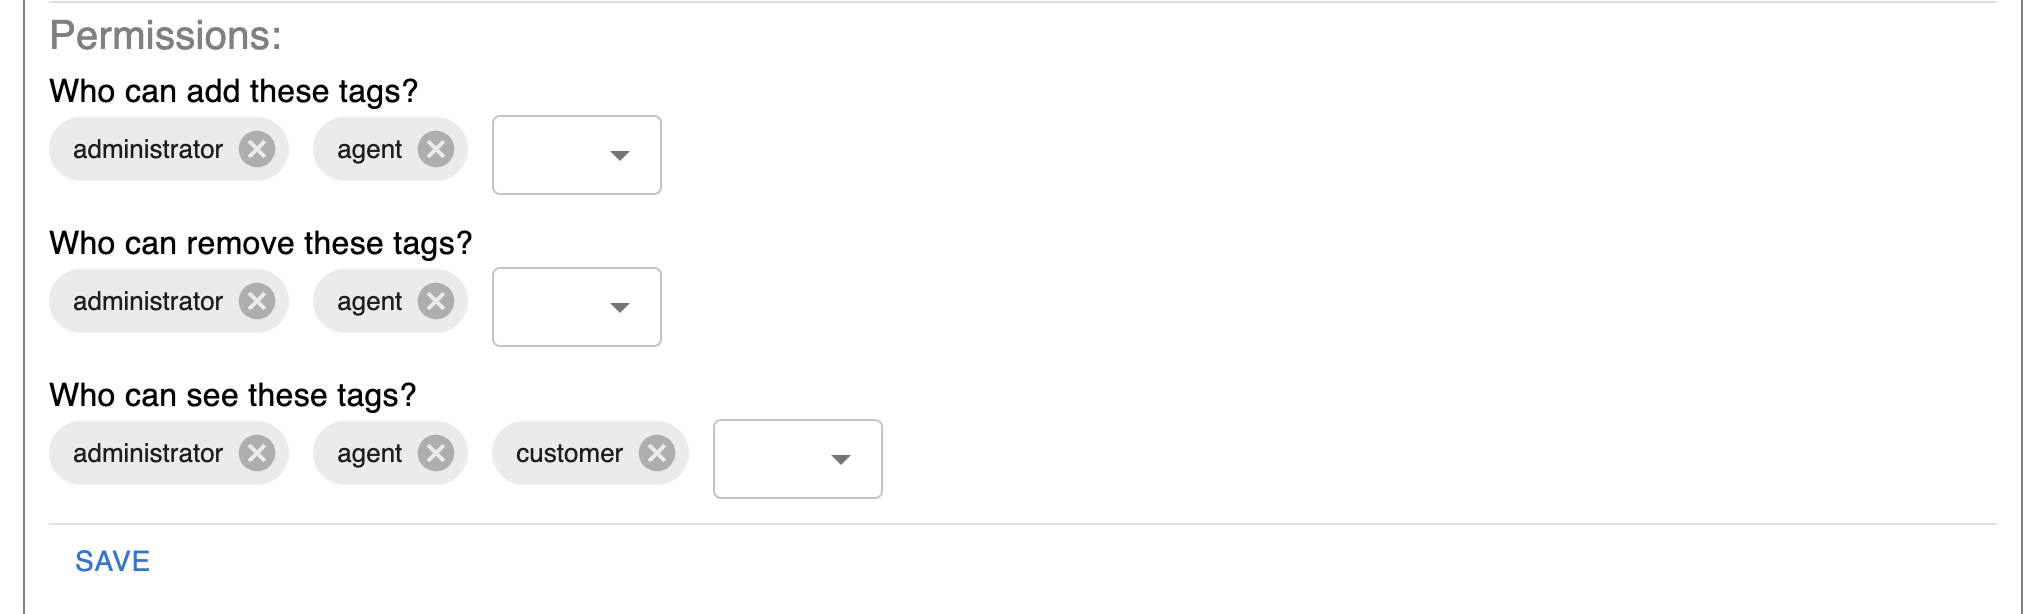
\includegraphics[width=1\textwidth]{docs/images/ch_1/tag-mgmt-permissions.png} 
  \caption{Kreiranje oznake, permisije.}
\end{figure}

\newpage
\subsection{Upravljanje korisnicima}

Administratori poseduju mogućnost upravljanja korisnicima sajta putem kontrolne table na adresi \verb|manage/users|. Tabla prikazuje listu svih korisnika i akcije koje mogu biti primenjene nad njima. Od akcija podržana je promena tipa korisnika (pod određenim uslovima) i promena statusa korisnika.

\begin{figure}[h]
  \centering
  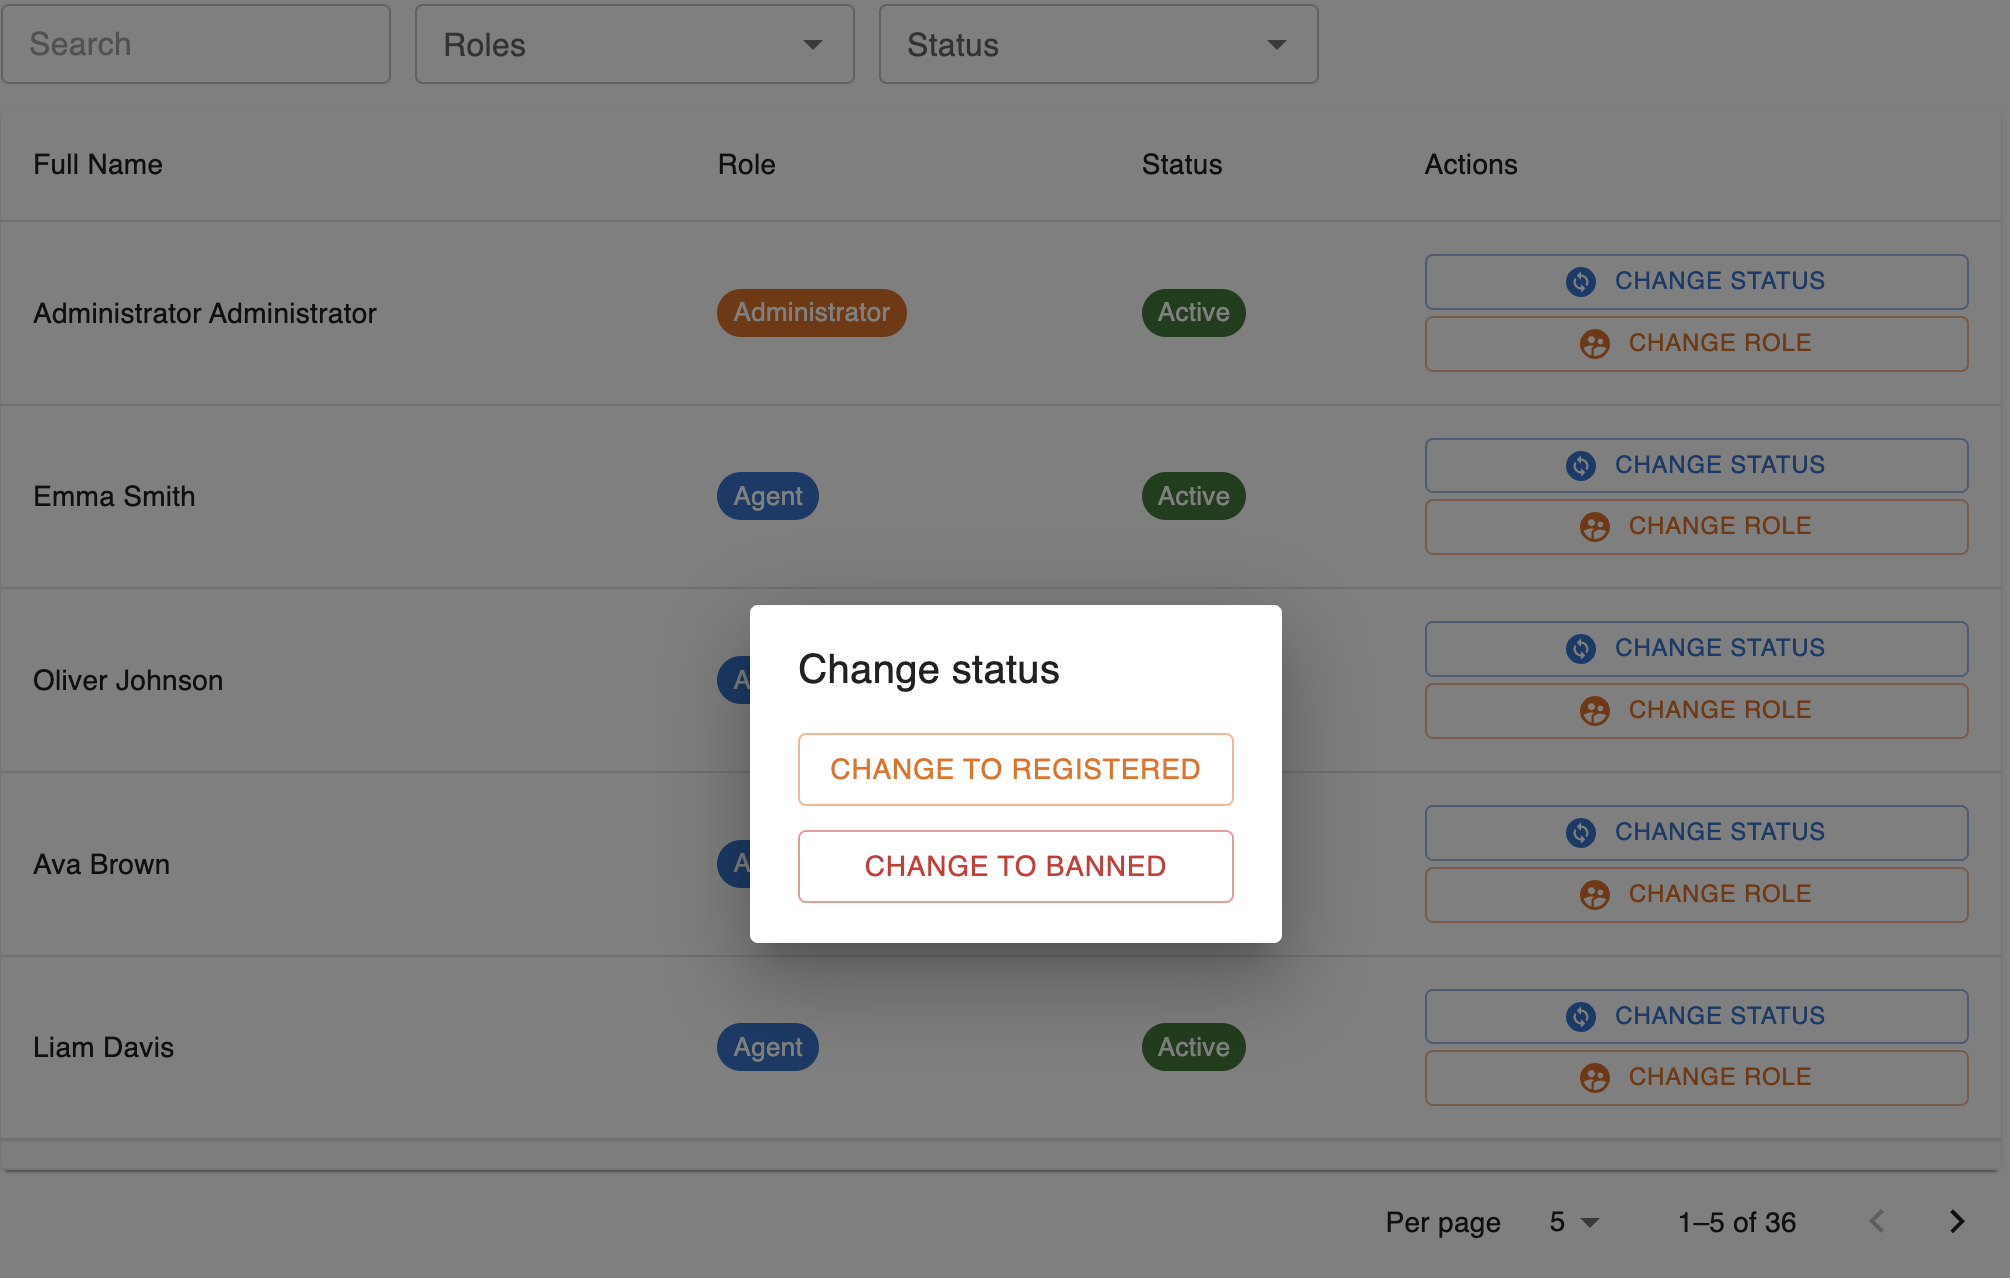
\includegraphics[width=1\textwidth]{docs/images/ch_1/manage-users-preview.png} 
  \caption{Upravljanje korisnicima.}
\end{figure}

\newpage
\subsection{Postavljanje kartice}

Na kraju, stranica na kojoj klijenti mogu postavljati nove kartice jednostavan je obrazac koji se sastoji iz naslova i tela kartice.

\begin{figure}[h]
  \centering
  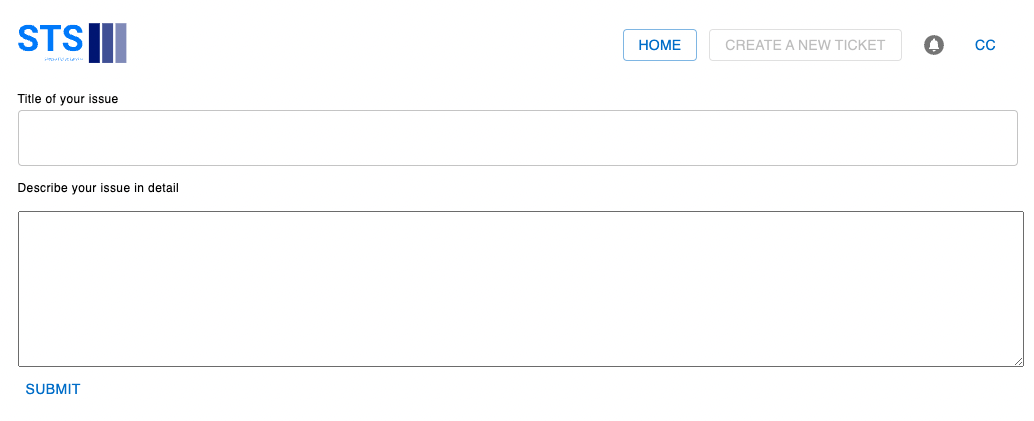
\includegraphics[width=1\textwidth]{docs/images/ch_1/ticket-new.png} 
  \caption{Kreiranje kartice.}
\end{figure}

\newpage



\section{Entiteti i njihovi odnosi, ER dijagram}

ER model\footnote{eng. Entity-relationship model - model entiteta i odnosa.} predstavlja jedan vid konceptualnog modelovanja podataka u softverskom sistemu \cite{dbmodelinganddesign}. Sam po sebi je apstraktan pojam bez vidljive reprezentacije, s tim što se često poistovećuje sa pojmom \textit{ER dijagrama} koji je notaciono sredstvo za prikaz modela nastalog ER modelovanjem.

Sastoji se od nekoliko vrsta elemenata:
\begin{itemize}
    \item \textbf{Entiteti} predstavljaju stvari iz realnog sveta koje se modeluju. Jedna pojedinačna pojava entiteta naziva se \textit{instanca entiteta} \cite{dbmodelinganddesign}. ER dijagram koristi pravougaonike za oznaku entiteta.
    \item \textbf{Odnosi} predstavljaju asocijacije između entiteta u najopštijem smislu. Karakteriše ih i brojnost koja pruža informaciju o broju instanci svakog entiteta u datom odnosu. Ovakav sistem poznat je i u modelovanju relacionih baza pod nazivima "1 na 1", "1 ka više" i "više ka više". ER dijagram koristi kvadrat za označavanje odnosa.
    \item \textbf{Atributi} jesu karakteristike entiteta ili odnosa koje pružaju dodatne detalje o njima. Atributi mogu biti ključni, u kom slučaju učestuvju u identifikaciji entiteta ili odnosa, ili deskriptivni, kada se odnose na nejedinstvene osobine \cite{dbmodelinganddesign}. Prikazuju se elipsama koje su strelicama povezane za entitet ili odnos kom pripadaju, dok se imena ključnih atributa podvlače.
\end{itemize}

ER modelovanje neretko se dovodi u vezu sa modelovanjem relacionih baza podataka. Model ipak nije ograničen na vrstu baze podataka, tako da se koristi i ovde  uprkos tome što je baza sistema nerelaciona - konkretno MongoDB. Štaviše, proces transformacije ER modela u dokumentni model dodatno je olakšan, jer za određene asocijacije nije potrebno praviti dodatne tabele/dokumente usled mogućnosti čuvanja kompleksnih polja u dokumentima. Na narednom dijagramu prikazan je uprošćen\footnote{Neki atributi nisu prikazani zbog kompaktnosti, neki odnosi korisnika i kartica nisu prikazani jer su jednostavni (promena naslova, promena tela).} ER dijagram sistema STS.

\begin{figure}[h]
  \centering
  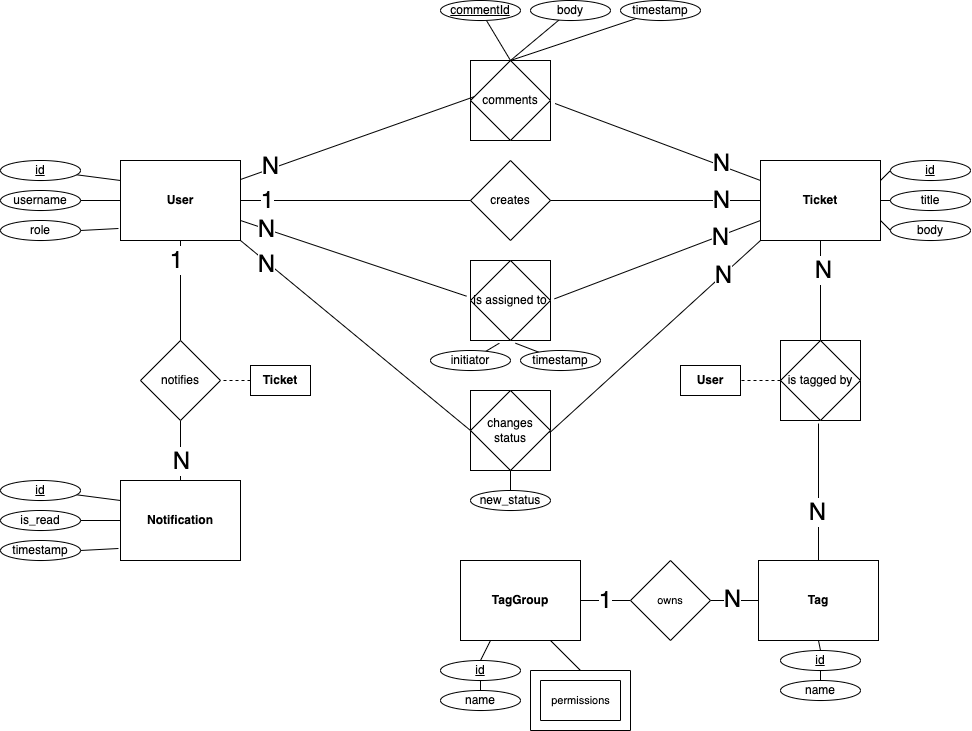
\includegraphics[width=1\textwidth]{docs/images/ch_1/rdiagram.png} 
  \caption{ER dijagram sistema STS.}
\end{figure}

\newpage
\subsection{Odnos kartica i korisnika, složeni odnosi}
Može se primetiti da dva glavna entiteta - kartica i korisnik - mogu biti u više različitih odnosa:
\begin{itemize}
    \item Korisnik može kreirati više kartica (odnos \verb|creates|), dok kartica može biti kreirana od strane samo jednog korisnika.
    \item Korisnik može komentarisati na karticu (odnos \verb|comments|). Vredno pomena je da ovaj odnos sadrži dodatne podatke, kao što su identifikator, telo i vreme komentara.
    \item Korisnik može biti dodeljen kartici (odnos \verb|is_assigned_to|), i tu dodelu može izvršiti drugi korisnik, označen atributom \verb|initiator|.
    \item Korisnik može menjati status kartice (odnos \verb|changes_status|).
\end{itemize}

Kompleksni odnosi, kao što su komentarisanje i dodeljivanje, u relacionoj bazi podataka morali bi biti izvedeni odgovarajućim zasebnim veznim relacijama. Na primer, u slučaju komentarisanja, ako bi korisnik i kartica bili predstavljani sledećim relacijama (koristeći relacionu notaciju):

\begin{center}
\textbf{Ticket}(\underline{id}, title, body, status, creator\_id)    
\end{center}

\begin{center}
\textbf{User}(\underline{id}, username, role)    
\end{center}

tada bi komentar zahtevao dodatnu relacija koja sadrži identifikator kartice i korisnika:

\begin{center}
\textbf{Comment}(\underline{comment\_id}, user\_id, ticket\_id, body, timestamp)    
\end{center}

Budući da se koristi MongoDB i dokumentni model podataka, moguće je komentare čuvati u okviru dokumenta kartice. Tačnije, u sloju baze podataka, ovi komentari se ne čuvaju eksplicitno, već kroz sistem istorije. Ukratko, svaka promena nad karticom se pamti kao jedan događaj u nizu \verb|history|, uz odgovarajući tip promene i neophodne podatke.

\begin{figure}[h]
\begin{lstlisting}[language=JavaScript, style=ES6, caption={Tip podataka istorije kartice.}]
export class TicketHistoryItem {
  timestamp: Date;
  initiator: UserDb;
  type: TicketHistoryEntryType;
  payload:
    | TicketHistoryEntryCreated
    | TicketHistoryEntryStatusChanged
    | TicketHistoryEntryCommentAdded
    | TicketHistoryEntryTitleChanged
    | TicketHistoryEntryBodyChanged
    | TicketHistoryEntryAssigneesChanged
    | TicketHistoryEntryTagsChanged
    | TicketHistoryEntryCommentChanged
    | TicketHistoryEntryCommentDeleted;
}
\end{lstlisting}
\end{figure}

O ovom sistemu iz domenskog ugla biće više reči u sekciji \ref{sec:eventsourcing}. Svakako, ER model sam po sebi ne propisuje način realizacije odnosa, jer nije vezan ni za jedan model baze podataka.

\subsection{Oznake i grupe oznaka, slabi entiteti}

Kao što je pomenuto u prethodnoj sekciji, uveden je fleksibilan sistem oznaka takav da je moguće upravljati samim sistemom bez intervencije programera. Oznake se mogu dodeljivati kartici, a same mogu pripadati grupi oznaka. Jedan očigledan primer upotrebe ovog sistema je označavanje koliko je data kartica hitna - grupa oznaka bila bi \textbf{hitnost}, dok bi konkretne oznake bile, primera radi, \textbf{veoma hitno}, \textbf{umereno hitno} i \textbf{nije hitno}.

Dodatni nivo fleksibilnosti postiže se ograničavanjem ko može koju akciju da vrši nad kojom grupom oznaka. Na primer, klijent koji postavlja karticu može videti kojom hitnošću je označeno njegovo pitanje, ali ne može sam označiti hitnost usled činjenice da se ne može smatrati objektivnim po tom pitanju. Ovim se uvodi još jedan element ER modela, prikazan na dijagramu pravougaonikom sa duplim ivicama, poznat kao \textbf{slab entitet}\footnote{eng. weak entity}. Uglavnom nastaju od kompleksnih atributa, odnosno atributa koji se ne mogu izraziti jednom vrednošću\footnote{Knjiški primer slabog entiteta je adresa - sastoji se od ulice i broja. Ipak, postoje situacije gde adresa može biti i (jak) entitet.} i odlikuje ih nedostatak sopstvenog identiteta - identitet slabog entiteta je "pozajmljen" od strane jakog entiteta kome pripada \cite{dbmodelinganddesign}. U ovom slučaju, slab entitet \textbf{dozvola} (eng. permissions) sastoji se od sledećih podataka:
\begin{itemize}
    \item lista uloga korisnika koji mogu da vide oznake iz date grupe
    \item lista uloga korisnika koji mogu da dodaju oznake iz date grupe
    \item lista uloga korisnika koji mogu da uklanjaju oznake iz date grupe
\end{itemize}

U domenskom sloju softverskog sistema, o kome će biti reči u sekciji \ref{sec:dddsection}, slabi entiteti se najčešće preslikavaju u pojam \textit{vrednosnih objekata}\footnote{eng. value objects}, dok se u k\^{o}du realizuju putem običnih klasa\footnote{U praksi postoji konvencija nazivanja takvih objekata kao \textit{Plain Old} (stari dobri) objekti. Tako u slučaju jezika Javascript nazivaju se POJO (Plain old Javascript Object), dok bi za PHP bili POPO, i sl.}.






% ------------------------------------------------------------------------------
\chapter{Bekend}
\label{sec:backend}
% ------------------------------------------------------------------------------
Kod velikog broja softverskih sistema serverski deo aplikacije (bekend) može se uopšteno shvatiti kao aplikacija koja apstrahuje pristup podacima na udaljenom serveru. Podaci se skoro uvek čuvaju u nekoj vrsti baze podataka, dok se pristup i manipulacija podacima dodatno apstrahuje aplikativnim\footnote{Opštosti radi, izbegnuti su pojmovi \textbf{veb server} i \textbf{http server}. Veb server predstavlja server za dostavljanje statičkog sadržaja na vebu, i često kada se govori o bekend aplikacijama ne misli se na ovaj tip servera (nginx, apache2). HTTP server takođe ne bi bio ispravan pojam usled postojanja drugih protokola komunikacije na vebu.} serverom.

Navedeni gradivni delovi - baza podataka i aplikativni server - tehnički su dovoljni za implementaciju bekend dela aplikacije. Mnogi kursevi razvoja veb aplikacija, pogotovu oni zasnovani na MEAN i MERN\footnote{Mongo, Angular ili React, Express, Node.js, dve popularne kombinacije veb tehnologija.} okruženjima, upravo ovakve primere i prikazuju. Tu se neretko sreće arhitektura od samo dva sloja - sloj aplikativnog programskog interfejsa (eng. Application Programming Interface - API) i sloja pristupa bazi podatka. Međutim, za izgradnju složene aplikacije koja uzima u obzir čistoću k\^{o}da, razdvajanje odgovornosti, održivost i iskustvo programera (eng. Developer Experience - DX) potrebno je dodatno raslojiti aplikaciju i pratiti neke ustanovljene principe.


\section{DDD}
\label{sec:dddsection}
Jedan od najpopularnijih pristupa za dizajn i modelovanje softvera jeste dizajn zasnovan na domenu (eng. Domain Driven Design - DDD). DDD zagovara detaljno upoznavanje svih učesnika razvoja softvera sa domenom koji dati softverski sistem predstavlja. Programeri u saradnji sa domenskim stručnjacima razvijaju zajednički, sveprisutan jezik (eng. ubiquitous language) kako bi se prevazišla barijera različitog rečnika svih strana. \cite{dddq}

\subsection{Korišćenje domenskog jezika u programskom k\^{o}du}
\label{sec:dddukodu}
Nakon uspostavljanja, sveprisutan jezik postaje sastavni deo komunikacije programera i domenskih stručnjaka (i svih ostalih učesnika razvoja), ali isto tako i programskog k\^{o}da. Naime, programski k\^{o}d koji nastaje kao produkt modelovanja principa DDD-a postaje jasniji i dostiže viši stepen samodokumentovanosti. U takvom k\^{o}du sama imena klasa, metoda i promenljivih mogu biti dovoljna da programeru daju jasnu sliku šta koja celina k\^{o}da radi. Upravo zbog ovoga, primena DDD-a nije ograničena samo na velike kompanije ili velike timove, i ne služi samo kao sredstvo prevazilaženja "jezičkih" barijera, već doprinosi čistoći k\^{o}da i arhitekture i u manjim timovima, čak i jednočlanim. U sledeća dva primera prikazan je deo metode koja vrši ažuriranje komentara na kartici. Primer \ref{lst:nonddd} prikazuje ovu metodu, ne uzimajuću domenski jezik u obzir.


\begin{figure}[h]
\begin{lstlisting}[language=JavaScript, style=ES6, caption={K\^{o}d koji nije na domenskom jeziku}, label={lst:nonddd}]
function updateComment(...){
  const ticket = //...
  
  if (!ticket) {
    throw new NotFoundException('Ticket not found.');
  }

  if (ticket.status === TicketStatus.CLOSED ||
      ticket.status === TicketStatus.RESOLVED) {
    throw new BadRequestException('Ticket closed.')
  }

  if (user.role === Role.CUSTOMER &&
      ticket.createdBy.id !== user.id) {
    throw new ForbiddenException('Not your ticket');
  }
  
  const comment = //...
  
  if (!comment) {
    throw new NotFoundException('Comment not found.')
  }
  
  if (comment.user.id !== user.id) {
    throw new ForbiddenException('Not your comment.');
  }
}
\end{lstlisting}
\end{figure}
\newpage
Odlikuje se ručnim proverama identifikacionih polja i direktnim podizanjem HTTP grešaka unutar servisa. Iako može biti razumljiv u toku pisanja, ovakva vrsta k\^{o}da u kompleksnom sistemu postaje neodrživa zbog nečitljivosti.

\begin{figure}[h]
\begin{lstlisting}[language=JavaScript, style=ES6, caption={K\^{o}d koji je na domenskom jeziku}]
function updateComment(...) {
  const ticket = // ...

  if (!ticket) {
    throw new TicketNotFoundError(ticketId);
  }

  if (ticket.isFinalStatus()) {
    throw new CannotChangeTicketInFinalStatusError(ticket.status);
  }

  if (user.isCustomer() && !ticket.isOwner(user)) {
    throw new CannotCommentOnOthersTicketsError();
  }

  const comment = // ...

  if (!comment) {
    throw new CommentNotFoundError();
  }

  if (!comment.isOwner(user)) {
    throw new CannotUpdateOthersCommentsError();
  }
}
\end{lstlisting}
\end{figure}

\newpage
U ovom primeru evidentno je prisustvo domena u svim aspektima. Metode kao što su \verb|isFinalStatus| i \verb|isOwner| i semantičke klase grešaka kao \verb|TicketNotFoundError| doprinose da određeni delovi k\^{o}da dostižu nivoe čitljivosti bliske prirodnom jeziku.

\subsection{Slojevita arhitektura}
Prilikom izrade softvera, usled rokova i nedostatka resursa, neretko dolazi do isprepletanosti poslovne logike, logike korisničkog interfejsa, logike pristupa bazi podataka i drugih komponenti sistema \cite{dddfull}. Ovakve odluke u razvoju, iako rezultuju kratkoročnim rešenjem, dugoročno dovode do borbe sa \textit{tehničkim dugom} (eng. technical debt). Postojanje tehničkog duga javlja se i iz drugih odluka tokom razvoja i u praksi je pokazano da opšte rešenje ovog problema ne postoji; svaki tim se pre ili kasnije sretne sa tehničkim dugom koji otežava i usporava rad. Ipak, ta neminovnost ne treba da obeshrabri rano uvođenje dobrih praksi kao što je raslojavanje arhitekture. 

DDD razaznaje četiri sloja, s tim što se ovo poglavlje odnosi na prva tri, dok je sloj korisničkog interfejsa predmet narednog poglavlja. Detaljna diskusija o slojevima, uz relevantnu implementaciju, prikazana je u sekcijama 2.2, 2.3 i 2.4.

\begin{figure}[h]
  \centering
  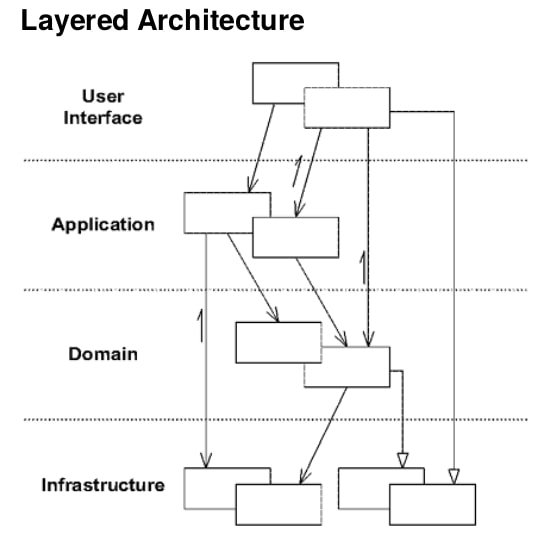
\includegraphics[width=0.5\textwidth]{docs/images/ch_2/DDD-Layered-Architecture-2.png} 
  \caption{Slojevi sistema \cite{dddfull}.}
  \label{fig:sample}
\end{figure}

\section{Okruženje NestJS}

NestJS \cite{nestjsdocs} je Node.js okruženje za razvoj serverskih aplikacija. Izgrađen je nad bibliotekom \verb|express| \cite{expressjsdocs} koja je i danas popularan izbor za izradu manjih serverskih aplikacija kao i za edukativne svrhe.  U srž ovog okruženja ugrađeni su koncepti modula, servisa i umetanja zavisnosti (eng. Dependency Injection - DI), što ga čini idealnim za konstrukciju aplikacije zasnovane na DDD principima.

Osnovni gradivni elementi NestJS aplikacije su \textit{moduli}. Svaki modul obuhvata jednu smislenu celinu aplikacije koja može sadržati \textit{kontrolere} i \textit{provajdere}. U slučaju DDD-a, modul odgovara jednom izolovanom kontekstu\footnote{eng. Bounded Context \cite{dddfull}}. Moduli se definišu na deklarativni način, pri čemu se u okviru modula mogu uvoziti i drugi moduli kako bi se postigla saradnja različitih delova sistema.

\begin{figure}[h]
\begin{lstlisting}[language=JavaScript, style=ES6, caption={Deklaracija modula za kartice.}]
@Module({
  // Sekcija koja uvozi ostale module
  imports: [
    MongooseModule.forFeature(...),
    UsersModule,
    TicketTagSystemModule,
    NotificationsModule,
  ],
  // Sekcija koja deklarise kontrolere
  controllers: [TicketsController],
  // Sekcija koja deklarise servise i repozitorijume
  providers: [
    TicketService,
    TicketCommentService,
    TicketRedactionService,
    TicketTagUpdateService,
    TicketAssigneesService,
    TicketsRepository,
  ],
})
export class TicketsModule {}
\end{lstlisting}
\end{figure}

Kao što se vidi u primeru, NestJS se u velikoj meri oslanja na metaprogramiranje i mogućnosti jezika \verb|typescript| u vidu dekoratora. Prilikom pokretanja NestJS aplikacije vrši se korak poznat kao \textbf{bootstrap}, odnosno priprema aplikacije za rad. U tom koraku se razrešavaju sve međuzavisnosti modula i servisa, i instanciraju sve klase kojima se upravlja putem umetanja zavisnosti.

Što se tiče strukture direktorijuma i fajlova u okviru projekta, iskorišćen je hibrid između mnogo sistema viđenih u praktičnom radu. Takva struktura najbolje odgovara zahtevima okruženja i sistema koji se modeluje. Primer strukture prikazan je u \ref{lst:dddfolderstructure}.

\begin{figure}[h]
\begin{lstlisting}[language=JavaScript, style=ES6, caption={fajl tickets.module.ts},label={lst:dddfolderstructure}]
|-- api/
|   |-- dto/
|   |-- profiles/
|-- domain
|   |-- entities/
|   |-- errors/
|   |-- services/
|   |-- value-objects/
|-- infrastructure
    |-- interceptors/
    |-- schema/
\end{lstlisting}
\end{figure}

\section{Sloj infrastrukture}

Sloj infrastrukture ima više uloga u DDD sistemu, ali zajednička osobina je odsustvo iniciranja akcija u sloju domena \cite{dddfull}. Veliki deo ovog sloja često zauzima implementacija trajnosti podataka (eng. data persistence), i to neretko šablonom repozitorijuma (eng. Repository pattern). Uloga ovog šablona jeste odvajanje logike za čuvanje podataka van domenskog modela \cite{msrepository}. Često se ostvaruje uz pomoć jedne ili više klasa sa nekim uobičajenim metodama za dohvatanje ili ažuriranje entiteta.


\subsection{Repozitorijumi}
Apstrakcija koju pruža sloj repozitorijuma ogleda se upravo u načinu na koji on obrađuje podatke pre vraćanja u više slojeve, tačnije služi se \textbf{šablonom preslikavanja podataka} (eng. Data mapper pattern). Uloga mapiranja podataka uglavnom je u praksi delegirana konkretnoj biblioteci ili okruženju, koje upravlja pristupom bazi putem softverskog segmenta iz klase Objektno-relacionih ili Objektno-dokumentnih preslikavača (eng. Object Relational Mapper - ORM, Object Document Mapper - ODM). Iako ti sistemi često u potpunosti zadovoljavaju potrebe mapiranja podataka, u ovom radu je mapiranje urađeno ručno, tako da se objekti dobijeni ODM slojem, odnosno bibliotekom \verb|mongoose| \cite{mongoosedocs}, preslikavaju u entitete koristeći biblioteku \verb|@automapper/js| \cite{automapperjsdocs}.

\begin{figure}[h]
  \centering
  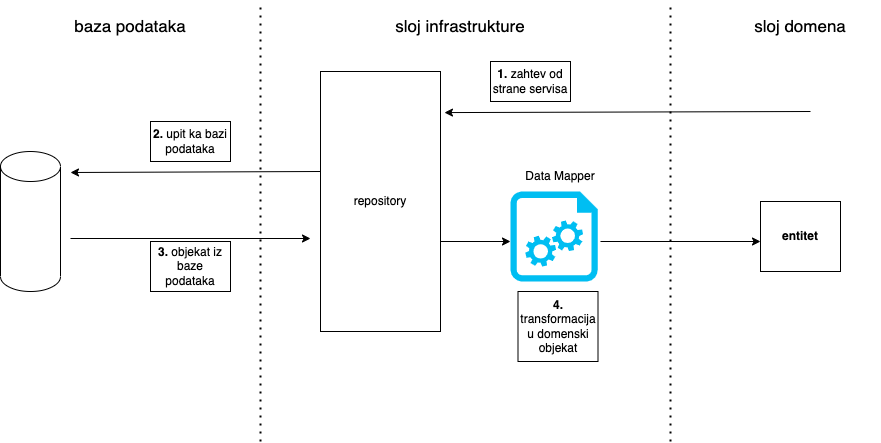
\includegraphics[width=1\textwidth]{docs/images/ch_2/repository.drawio.png} 
  \caption{Dijagram dohvatanja entiteta preko repozitorijuma.}
  \label{fig:sample}
\end{figure}

Prirodno se nameće pitanje dohvatanja povezanih entiteta, ili konkretnije rad sa agregatima. U ovom radu implementiran je sistem \textbf{pohlepnog učitavanja} (eng. eager loading), kojim se svi povezani entiteti zahtevanog entiteta dohvataju odmah prilikom zahteva ka glavnom entitetu. U nekim sistemima ovakav izbor ne bi bio idealan, međutim takva odluka doneta je usled činjenice da je dizajn baze podataka relativno jednostavan, a lakoća implementacije i korišćenja nadmašuje cene u performansama koje su minimalne. Kombinacijom metode $populate$ 
 iz biblioteke \verb|mongoose|, kao i rekurzivne prirode biblioteke \verb|automapper/js|, ovo se lako postiže.

Primer \ref{lst:repositoryhead} prikazuje zaglavlje klase \verb|TicketsRepository|. Kao i sve ostale repozitorijumske klase, oslanjaju se na model klase dobijene od strane biblioteke \verb|mongoose| i deklarišu niz koji predstavlja sve putanje koje treba popuniti zarad implementacije pohlepnog učitavanja.

\begin{figure}[h]
\begin{lstlisting}[language=JavaScript, style=ES6, caption={Repozitorijum kartica, konstrukcija i niz POPULATE.}, label={lst:repositoryhead}]
export class TicketsRepository {
  constructor(
    @InjectModel() private ticketModel: Model<TicketDb>,
    @InjectMapper() private readonly mapper: Mapper,
  ) {}

  public static POPULATE = [
    {
      path: 'history.initiator',
      model: 'UserDb',
    },
    {
      path: 'history.payload.assignees',
      model: 'UserDb',
    },
    { path: 'createdBy', model: 'UserDb' },
    {
      path: 'tags',
      model: 'TicketTagDb',
      populate: { path: 'group', model: 'TicketTagGroupDb' },
    },
    { path: 'assignees', model: 'UserDb' },
  ];
\end{lstlisting}
\end{figure}

\newpage
Primer \ref{lst:repofetch} prikazuje primer dohvatanja jedne kartice putem identifikatora, pri čemu se, naravno, prilikom vraćanja rezultata vrši mapiranje u odgovarajući entitet.

\begin{figure}[h]
\begin{lstlisting}[language=JavaScript, style=ES6, caption={Dohvatanje jednog entiteta.},label={lst:repofetch}]
async findById(id: string): Promise<Ticket | null> {
    const result = await this.ticketModel
      .findById(id)
      .populate(TicketsRepository.POPULATE);
    
    if (!result) {
      return null;
    }
    
    return this.mapper.map(result, TicketDb, Ticket);
}
\end{lstlisting}
\end{figure}

\newpage
\subsection{Sheme, mutacije podataka, šablon Event Sourcing}
\label{sec:eventsourcing}
Osim repozitorijuma, sloj infrastrukture prirodno sadrži i definicije shema biblioteke \verb|mongoose|. Iz ugla programera, ovi objekti su najbliža pristupna tačka bazi podataka i podržavaju operacije upita i mutacija nad realnim podacima u bazi. Takav jedan upit viđen je na isečku \ref{lst:repofetch} u prethodnoj sekciji.

Na ovom mestu reč je o mutacijama podataka, i to baš kartica. Osim prikaza rada sa mutiranjem podataka kroz biblioteku \verb|mongoose|, ovaj primer služi da ilustruje dualnu prirodu kartice kao entiteta i njegovu potpunu različitost u strukturi između sloja infrastruktura i sloja domena. Naime, kao što će biti prikazano u sledećem poglavlju, kartica u sloju domena je jednostavna klasa koja sadrži sve podatke o datoj kartici. Ipak, u sloju infrastrukture, a radi veće fleksibilnosti i mogućnosti praćenja istorije, upotrebljena je varijanta šablona \textit{Event Sourcing}. Osnovno načelo ovog šablona je da se umesto čuvanja eksplicitnog stanja objekta čuva istorija njegovih promena.

Na isečku \ref{lst:ticketschema} prikazan je deo klase koja predstavlja shemu za rad sa karticama.

\begin{figure}[h]
\begin{lstlisting}[language=JavaScript, style=ES6, caption={Definicija sheme kartica.}, label={lst:ticketschema}]
@Schema({ collection: "tickets" })
export class TicketDb extends Document {
  _id: string;

  @Prop({ type: Date })
  createdAt: Date;

  @Prop({ type: String })
  title: string;

  @Prop({ type: String })
  body: string;

  @Prop({ type: String })
  status: TicketStatus;

 // ...

  @Prop({ type: [{ type: mongoose.Schema.Types.Mixed }] })
  history: TicketHistoryItem[];
}
\end{lstlisting}
\end{figure}


\newpage
Niz \verb|history| predstavlja promene primenjene na datoj kartici na osnovu kojih se može izvesti trenutno stanje kartice. Ipak, prirodno se postavlja pitanje zašto se, osim istorije promena, čuvaju i eksplicitna polja kao što su \verb|status|, \verb|title|, \verb|body| i drugi, budući da se ti podaci mogu izvući putem istorije. Razlog leži u performansama pretrage. Čuvanje samo liste promena, a ne slike trenutnog stanja (eng. snapshot), izazvalo bi da svaka pretraga bude linearne vremenske složenosti u odnosu na dužinu istorije, što bi rezultovalo lošim performansama.

Sa ovakvom postavkom, mutacije nad katicom postižu se diferencijacijom prosleđenog entiteta i entiteta iz baze podataka (primer \ref{lst:repodiff}).

\begin{figure}[h]
\begin{lstlisting}[language=JavaScript, style=ES6, caption={Fajl \textit{ticket.repository.ts}}, label={lst:repodiff}]
  async update(newTicket: Ticket, user: User) {
    const document = await this.ticketModel
      .findById(newTicket.id)
      .populate(TicketsRepository.POPULATE); 

    const timestamp = new Date();

    // Trenutno stanje kartice
    const ticket = this.mapper.map(document, TicketDb, Ticket);

    // Primer diferencijacije nad poljem title
    if (newTicket.title !== ticket.title) {
      const item = new TicketHistoryItem();
      item.initiator = user.id as unknown as UserDb;
      item.timestamp = timestamp;
      item.type = TicketHistoryEntryType.TITLE_CHANGED;

      // Dodaje se nova stavka u istoriju
      item.payload = 
         new TicketHistoryEntryTitleChanged(newTicket.title);
         
      document.history.push(item);
      // Menja se snapshot stanje
      document.title = newTicket.title;
    }
\end{lstlisting}
\end{figure}


\newpage
Za kraj, primer \ref{lst:mappingdata} prikazuje uprošćenu verziju mapiranja iz oblika u sloju infrastrukture u domenski entitet, dok se puna verzija nalazi u izvornom k\^{o}du u fajlu \verb|ticket.entity-profile.ts|.

\begin{figure}[h]
\begin{lstlisting}[language=JavaScript, style=ES6, caption={Mapiranje komentara kartice.}, label={lst:mappingdata}]
  forMember((destination) => destination.comments,
    mapFrom((source) => {
      const commentItems = source.history.filter(
        (item) => item.type === COMMENT_ADDED,
      );

      return commentItems
        .map((item) => {
          // pretrazuju se svi komentari u istoriji
          const payload = item.payload as CommentAdded;
          // proverava se da li su kasnije bili obrisani
          const deletes = source.history.filter(
            (deleteItem) => deleteItem.type === COMMENT_DELETED 
            && (deleteItem.payload as CommentDeleted)
                .commentId === payload.commentId,
            );
          
          const wasDeleted = deletes.length > 0;

          if (wasDeleted) {
            return null;
          }

          // ... mapiranje samog komentara u domenski oblik...

          return comment;

\end{lstlisting}
\end{figure}



\newpage
\section{Sloj domena}

Sloj domena sadrži glavnu poslovnu logiku i operacije koje direktno oslikavaju dešavanja u svetu koji softver modeluje. Iz ugla implementacije, svoje mogućnosti pružaju putem apstrakcije često nazivanom servisima, što se koristi i kao sufiks u nazivima njihovih klasa, iako se mogu koristiti i druge konvencije\footnote{Nekada se umesto sufiksa \textit{Service} koriste reči koje direktno oslikavaju namenu datog servisa. Na primer umesto \textit{GetUserService} koristi se naziv \textit{UserProvider} i sl.}.

\subsection{Tok podataka kroz domenski sloj}

Usled činjenice da obuhvata sve poslovne operacije nije lako definisati opštu namenu domenskog sloja. Na slici \ref{fig:domainlayerdiagram} prikazan je uopšten primer toka podataka kroz ovaj sloj i njemu susedne slojeve.

\begin{figure}[h]
  \centering
  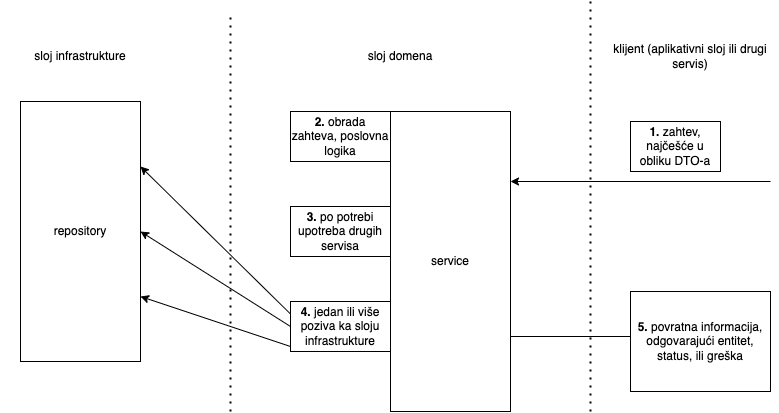
\includegraphics[width=1\textwidth]{docs/images/ch_2/domain.png} 
  \caption{Uopšteni tok obrade podataka kroz domenski sloj.}
  \label{fig:domainlayerdiagram}
\end{figure}

Ipak, operacije unutar servisa (koraci 2-4) konkretizovane su za potrebe sistema koji se razmatra, jer se mogu svesti na sledeći šablon, gde redosled ne mora nužno biti ispraćen u k\^{o}du usled prirode jezika\footnote{Zbog asinhrone prirode okruženja Node.js, a radi postizanja maksimalnih performansi, neke operacije pokreću se paralelno a zatim čekaju koristeći funkciju $Promise.all$, što može naizgled delovati kao mešanje koraka.}:

\begin{enumerate}
  \item Dohvatanje odgovarajućeg entiteta
  \item Provera domenskih prava pristupa i domenskih grešaka
  \item Obrada entiteta
  \item Komunikacija sa drugim servisima
  \item Osiguravanje trajnosti podataka
  \item Priprema i vraćanje odgovarajućeg odgovora
\end{enumerate}

Na sledećem primeru operacije dodeljivanja kartice agentima prikazani su prethodni koraci, redom.

\textbf{Dohvatanje entiteta}

\begin{figure}[h]
\begin{lstlisting}[language=JavaScript, style=ES6, caption={Korak dohvatanja kartice.}]
async addAssignees(ticketId: string, user: User, dto: AssignDTO) {
  const ticket = await this.ticketsRepository.findById(ticketId);
  if (!ticket) {
    throw new TicketNotFoundError(ticket.id);
  }
\end{lstlisting}
\end{figure}

\textbf{Provera domenskih prava pristupa i domenskih grešaka}
\begin{figure}[h]
\begin{lstlisting}[language=JavaScript, style=ES6, caption={Korak provere domenskih prava pristupa i domenskih grešaka.}]
  // Domensko pravo pristupa - korisnicima nije dozvoljeno
  // dodeljivanje kartica
  if (user.isCustomer()) {
    throw new NotAllowedToAssignError();
  }
  const assignees: User[] = await Promise.all(
    dto.assignees.map((id) => this.usersService.findOne(id)),
  );

  for (const assigneeUser of assignees) {
    // Greske domenskog karatkera
    if (!assigneeUser) {
      throw new AssigneeNotFoundError();
    }
    if (assigneeUser.isCustomer()) {
      throw new CannotAssignCustomerError(assigneeUser.id);
    }
    if (ticket.isAssigned(assigneeUser)) {
      throw new DuplicateAssigneeError(assigneeUser.id);
    }
}
\end{lstlisting}
\end{figure}

\newpage
\textbf{Obrada entiteta}

U ovom slučaju obrada je jednolinijska, zbog pogodne definicije klase Ticket.
\begin{figure}[h]
\begin{lstlisting}[language=JavaScript, style=ES6, caption={Korak obrade entiteta.}]
ticket.assign(assignees);
\end{lstlisting}
\end{figure}

\textbf{Komunikacija sa drugim servisima}

Konstruiše se niz obaveštenja koja je potrebno poslati, a slanje se delegira odgovarajućem servisu.
\begin{figure}[h]
\begin{lstlisting}[language=JavaScript, style=ES6, caption={Korak komunikacije sa drugim servisima.}]
const usersToNotify = assignees.filter(
  (assignee) => assignee.id !== user.id,
);
const notifications = usersToNotify.map((userToNotify) =>
  NotificationFactory.create((builder) =>
    builder
      .forUser(userToNotify)
      .hasPayload('assigned', (assignBuilder) =>
        assignBuilder.atTicket(ticket).byUser(user),
      ),
  ),
);
const promise = this.notificationsService.emitNotifications(
  ...notifications,
);
\end{lstlisting}
\end{figure}

\textbf{Osiguravanje trajnosti podataka}

Čuvaju se načinjene promene u bazi podataka.
\begin{figure}[h]
\begin{lstlisting}[language=JavaScript, style=ES6, caption={Korak očuvanja trajnosti podataka.}]
// ...
this.ticketsRepository.update(ticket, user);
\end{lstlisting}
\end{figure}

\newpage
\textbf{Priprema i vraćanje odgovarajućeg odgovora}

Gde se pritom koristi servis \verb|TicketRedactionService| zarad otklanjanja podataka koje dati tip korisnika ne bi trebalo da vidi.
\begin{figure}[h]
\begin{lstlisting}[language=JavaScript, style=ES6, caption={Korak pripreme i vraćanja odgovora.}]
this.ticketRedactionService.prepareResponse(updatedTicket, user);
return updatedTicket;
\end{lstlisting}
\end{figure}

\newpage
\subsection{Obrada grešaka}

U prethodnom primeru toka podataka javlja se intenzivan rad sa greškama. Ovom delu posvećena je posebna pažnja jer je obrada grešaka jedno od centralnih pitanja dizajna kompleksnog softverskog sistema, i bitno je od početka dizajnirati je korektno kako bi kasniji rad bio znatno olakšan.

Naime, programer koji se bavi implementacijom odgovarajuće domenske funkcionalnosti pre ili kasnije susrešće se sa potrebom da obrađuje greške. Čak i najjednostavniji zahtev, kao što je, recimo, dohvatanje jedne kartice, zahteva rad sa greškama na svakom od nivoa slojevite arhitekture. Manuelno orkestriranje grešaka pri svakoj implementaciji neke funkcionalnosti dovelo bi do usporenog rada i nekonzistentnog sistema bez jasnih standarda. 

Stoga se pravi jasna podela između grešaka domenskog nivoa i grešaka aplikativnog nivoa (HTTP grešaka), i u domenskom sloju radi se isključivo sa grešakama domenskog nivoa. Sve domenske greške nasleđuju baznu klasu $BaseError$ prikazano u primeru \ref{lst:baseerror}.

\begin{figure}[h]
\begin{lstlisting}[language=JavaScript, style=ES6, caption={BaseError.ts}, label={lst:baseerror}]
export class BaseError {
  constructor(public message: string = 'An error occurred') {}

  public getName() {
    return this.constructor.name;
  }

  public getPayload(): any {
    return {
      message: this.message,
      errorType: this.getName(),
    };
  }
}
\end{lstlisting}
\end{figure}

Na ovaj način realizovan je uniforman interfejs koji propisuje kako svaka greška treba da izgleda, sa dovoljno fleksibilnosti da pokrije sve domenske situacije. U k\^{o}du se može primetiti sve od jednostavnih grešaka koje predstavljaju nepostojanje - primer \verb|TicketNotFound|, do grešaka koje ukazuju na kompleksnu sitaciju - primer \verb|CannotChangeCommentsOfAClosedTicket|. Na ovakav sistem mogu se uložiti nekoliko kritika, koje su razmotrene u nastavku.

\textbf{Repetitivnost.}  
Sve greške koje se odnose na nepostajanje entiteta imaju identičan oblik, pa se može uložiti primedba na ponavljanje k\^{o}da i sugerisati kreiranje dodatnih apstrakcija. U ovom radu izbegnut je takav pristup iz dva razloga:
\begin{itemize}
    \item \textbf{Bespotrebne apstrakcije}. Iako je tehnički moguće apstrahovati greške nepostajanja entiteta u neki tip višeg nivoa - recimo \verb|EntityNotFoundError|, ovo uvodi previše jezičke kompleksnosti u domenski sloj i na duge staze ne doprinosi ni čitljivosti ni razumevanju.
    \item \textbf{Fleksibilnost}. Ukoliko svaki entitet ima priliku da definiše svoje greške bez ograničenja međuapstrakcija, postiže se maksimalna fleksibilnost u okviru datog entiteta. Može se argumentovati da ovakav pristup olakšava potencijalni prelaz na mikroservisnu arhitekturu, po potrebi.
\end{itemize}


\textbf{Preterana ekspresivnost.} Na ovom mestu konkretna primedba bila bi na račun dužine naziva nekih klasa, koje se mogu smatrati nečitljivim. Ipak, uzevši u obzir deo \ref{sec:dddukodu}, dobitak na razumljivosti domena kroz k\^{o}d nadmašuje strah od dugačkih imena klasa.


Ostaje pitanje transformacije ovakvih grešaka u HTTP oblik. Jedno izrazito elegantno rešenje, pruženo od strane okruženja NestJS, biće prikazano u sledećem pogavlju.

\section{Sloj aplikacije}

Svi do sad razmatrani sloji i delovi sistema mogu se smatrati internim u smislu mogućnosti spoljnjeg pristupa - sloj domena bavi se poslovnom logikom, uz podršku sloja infrastrukture. Kako bi domenski sistem mogao da se koristi od strane grafičkih veb aplikacija, mobilnih aplikacija ili, uopšteno, bilo kojih drugih softverskih sistema, potebno je da svoju funkcionalnost eksponira spoljašnjem svetu. 

\subsection{REST API, svojstva}
\label{sec:restapi}

Ispoljavanje spoljašnjem svetu postiže se slojem aplikacije, tankim slojem bez poslovnog znanja, čija glavna uloga jeste primanje zahteva i njihova delegacija na domenski sloj \cite{dddfull}. U ovom radu, za potrebe implementacije aplikativnog sloja, izabran je najpoznatiji arhitekturalni stil poznat kao REST (\textit{\textbf{RE}presentational \textbf{S}tate \textbf{T}ransfer}). Kompletna specifikacija ovog protokola je ogromna i pokriva sve aspekte korišćenja HTTP-a kao transportnog sloja veb aplikacija, tako da su u nastavku prikazane samo neke od najvažnijih osobina:

\begin{itemize}
    \item \textbf{Odsustvo stanja.} Jedan moderan princip softverskog inženjerstva (u vreme pisanja ovog rada) jeste da komponente ili moduli sistema treba da imaju što manje stanja, a po mogućstvu da ga u potpunosti eleminišu\footnote{Ovaj princip postaje posebno primetan rastom popularnosti funkcionalnih programskih jezika.}. Interpretacija u REST sistemima je sledeća - za dva API zahteva pod identičnim uslovima dobija se identičan odgovor. Dakle, ne postoji nikakav eksterni faktor samog aplikativnog sloja koji može uticati na odgovor koji korisnik (klijent) dobije, i smatra se da je klijent dužan da pruži kompletan kontekst potreban za obradu zahteva \cite{restapi}.

    \item \textbf{Identifikacija resursa i HTTP metode.} Neretko se u praksi sreću API slojevi sa previše ekspresivnim delovima URI-a\footnote{eng. Uniform Resource Identifier - URI}. REST definiše nedvosmislen način za identifikaciju resursa i njihovu hijerarhiju, kao i pravilnu upotrebu HTTP metoda (glagola). Na taj način API pristupna tačka\footnote{eng. API endpoint}, koja pruža mogućnost dohvatanja korisnika po identifikatoru, po pravilu treba da bude dostupna putem GET metode, i to na URI-u nalik na \verb|api/users/123| \cite{restapi}. Primer nepravilnog URI-a bilo bi direktno navođenje akcije dohvatanja - \verb|api/get-user-by-id/213|. Na sličan način jasno je propisano koje metode se koriste za promenu, upis i brisanje entiteta.

    \item \textbf{Korišćenje HTTP greški.} Kao što je pomenuto u prethodnoj sekciji, obrada grešaka predstavlja vitalan aspekt razvoja softvera, i značajan deo njene implementacije leži u aplikativnom sloju. REST definiše skup pravila za korektno ukazivanje korisniku na greške koje su se dogodile.  
\end{itemize}

\subsection{Kontroleri, validacija, mapiranje}

Većina okruženja za programiranje veb aplikacija, uključujući i NestJS, pruža ugrađen konstrukt za obradu HTTP zahteva poznat pod nazivom \textbf{kontroler}. Kontroleri su ništa drugo nego klase nad kojim se definišu metode koje obrađuju HTTP zahteve ka određenom URI-u, dok je proces mapiranja URI-a na metodu maksimalno prepušten okruženju, a programeru eksponiran nekim vidom metaprogramiranja (najšće dekoratorima). Primer \ref{lst:userscontroller} ilustruje kontroler vezan za URI prefiks \verb|users|, sa metodom koja reagovanje na dinamički zadat identifikator. Ovako postavljen kontroler obrađuje zahteve oblika \verb|GET /api/users/123|.

\begin{figure}[h]
\begin{lstlisting}[language=JavaScript, style=ES6, caption={Primer kontrolera.}, label={lst:userscontroller}]
@Controller('users')
export class UsersController {
  @Get(':id')
  findOne(id: number): UserDTO {
    // ...
  }
}
\end{lstlisting}
\end{figure}

Uloga kontrolera je višestruka i sastoji se od sledećih koraka:
\begin{enumerate}
    \item \textbf{Provera prava pristupa}. Ova provera treba da poznaje što manje poslovne logike. Na primer, neke pristupne tačke dostupne su samo ulogovanim korisnicima, neke samo administratorima, i sl.
    \item \textbf{Validacija ulaznih podataka}. Ponovo se misli na čisto tehničku validaciju, a ne na poslovnu validaciju. Tu spada provera da li su određeni brojčani podaci zaista brojevi, da li su određeni tekstualni podaci dovoljne dužine i slično.
    \item \textbf{Delegacija posla odgovarajućem sevisu}. Nakon uspešne provere prava pristupa i validacije podataka, kontroler će prepustiti zadatak servisu koji je za to namenjem i po potrebi primiti povratnu informaciju.
    \item \textbf{Obrada servisnih grešaka.} Kontroler je dužan da greške domenskog nivoa, koje podiže servis, preslika u HTTP greške. Neretka, i sasvim validna praksa, jeste korišćenje \verb|try-catch| blokova u ove svrhe. Ipak, vrlo elegantan mehanizam presretača (eng. interceptors) okruženja NestJS omogućio je izolaciju ovog posla. Naime, presretač je klasa koja se postavlja na nivo kontrolera, u kojoj se može dodati logika obrade grešaka podignutih iz domenskog sloja.
    \item \textbf{Preslikavanje podataka.} Ukoliko odgovor od servisa obuhvata entitet, dužnost kontrolera je da izvrši mapiranje datog entiteta u odgovarajući objekat za transfer podataka (eng. Data Transfer Object - DTO).
\end{enumerate}

Slika \ref{fig:applayerdiagram} prikazuje dijagram rada aplikativnog sloja.

\begin{figure}[h]
  \centering
  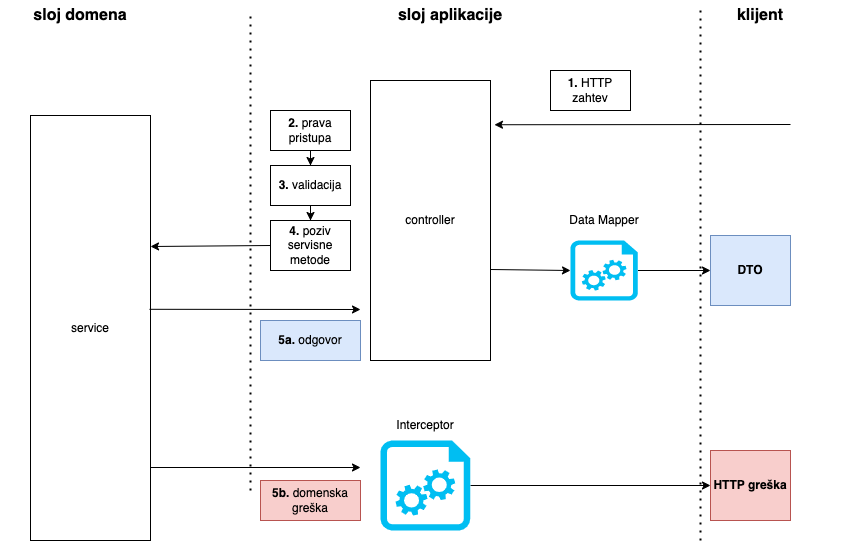
\includegraphics[width=1\textwidth]{docs/images/ch_2/applayer.png} 
  \caption{Aplikativni sloj.}
  \label{fig:applayerdiagram}
\end{figure}

Što se tiče tehničkih aspekata, maksimalno je korišćeno metaprogramiranje za postizanje validacije i preslikavanja grešaka, kako bi se izbeglo repetitivno pisanje k\^{o}da. Presretači su suštinski manuelne provere tipa instance greške. Validacija je izvedena deklarativno, kombinacijom biblioteka \verb|class-transformer| i \verb|class-validator|.

\begin{figure}[h]
\begin{lstlisting}[language=JavaScript, style=ES6, caption={Presretač grešaka.}]
return next.handle().pipe(
  catchError((error) => {
  if (error instanceof TicketNotFoundError) {
    throw new NotFoundException(error.getPayload());

    if (error instanceof NotAllowedToRemoveThisTagError) {
      throw new ForbiddenException(error.getPayload());
    }

    if (error instanceof DuplicateTagError) {
      throw new ConflictException(error.getPayload());
    }
\end{lstlisting}
\end{figure}




\begin{figure}[h]
\begin{lstlisting}[language=JavaScript, style=ES6, caption={Validacija ulaznog DTO-a.}]
export class AddTicketTagsDTO {
  @Validate(isValidObjectId, { each: true })
  @IsArray()
  tags: string[];
}
\end{lstlisting}
\end{figure}




    






% ------------------------------------------------------------------------------
\chapter{Frontend}

Ukoliko bi tražili jedan programski jezik koji može da pokrije najširi spektar platformi i aplikacija, to bi u današnje vreme definitivno bio Javascript. Uprkos velikom broju platformi koje mogu pokretati Javascript k\^{o}d (veb pregledači, Node.js, Deno, Bun, itd), glavno okruženje koje diktira njegov razvoj jeste upravo i originalno - veb. Pod ovim se misli na podudaranje između Javascript-a definisanog prema TC39\footnote{eng. Technical committee 39 - tehnički komitet zadužen za standardizovanje jezika.} standardu i Javascript-a koji se izvršava u veb pregledačima \cite{ydkjs}. Postojanje tolikog broja okruženja prirodno je dovelo do alata, ili čak kompletnih okruženja za razvoj, sa ciljem da apstrahuju sistem nad kojim se izvršava i da k\^{o}d učine što univerzalnijim.


\section{Kratak pregled evolucije jezika Javascript i frontend razvoja}

\subsection{Statički sajtovi}
Prvi oblik veb sajtova bio je veoma jednostavan. Zasnivao se na konceptu dostavljanja statičkih HTML i CSS fajlova preko kojih je korisnik mogao da pregleda neki sadržaj. Navigacija se vršila kroz hiperlinkove koji bi upućivali na druge adrese gde bi klijent zahtevao druge statičke fajlove, čime bi proces počinjao ponovo.

\begin{figure}[h]
  \centering
  
\includegraphics[width=0.7\textwidth]{docs/images/ch_4/frontend-dev-phase0.png} 
  \caption{Dostavljanje statičkih HTML sajtova.}
  \label{fig:sample}
\end{figure}

\subsection{Dodavanje klijentske interaktivnosti}

Problem koji se javlja sa prethodnim sistemom jeste nedostatak klijentske interaktivnosti - za svaku promenu sadržaja stranice potrebno je učitati celu stranicu od početka\footnote{Najbolji primer koji ilustruje probleme nedostatka interaktivnosti jesu veliki formulari i njihova validacija. Na modernim veb sajtovima prilikom popunjavanja velikih formulara korisnik konstantno ima povratnu informaciju da li je neko polje pogrešno popunjeno, dok pre Javascript-a to se saznaje tek nakon podnošenja.}. Uvođenje klijentskih skripti jezikom Javascript omogućuje se manipulacija HTML elemenata sa klijentske strane, upravljanje događajima, i slično.

\begin{figure}[h]
  \centering
  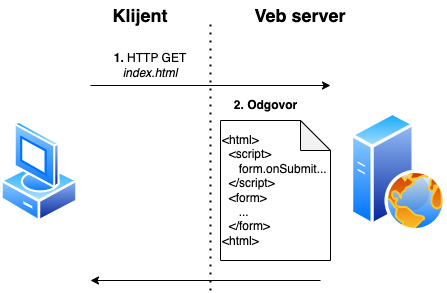
\includegraphics[width=0.7\textwidth]{docs/images/ch_4/frontend-dev-phase1.png} 
  \caption{Dostavljanje statičkih HTML sajtova i propratnih skripti.}
  \label{fig:sample}
\end{figure}

\newpage
\subsection{Jednostranične aplikacije - SPA}

Sledeći veliki zaokret dešava se uvođenjem koncepta jednostraničnih aplikacija (eng. Single Page Application - SPA). Ove aplikacije odlikuje potpuno prebacivanje logike generisanja korisničkog interfejsa na frontend deo aplikacije. Server bi poslao samo skelet HTML-a i Javascript skriptu, koja bi zatim preuzela odgovornost prikaza elemenata. Dohvatanje podataka (eng. data fetching) za prikaz na stranici vršilo bi se putem API-a, tako da ovaj sistem podseća na način na koji rade mobilne aplikacije - potpuno razdvajanje odgovornosti prikaza korisničkog interfejsa i dohvatanja podataka. Originalne mane ovakvog sistema zasnivale su se na lošijem rangiranju stranica od strane sistema za pretragu usled manjka početnog sadržaja koji se prikazuje\footnote{U današnje vreme skoro svi moderni pretraživači uspešno indeksiraju i SPA sajtove, tako da je ovaj problem praktično eleminisan.}. Prednost je u korisničkom iskustvu - navigacija se vrši potpuno klijentski tako da korisnik ima osećaj jako brze navigacije, kao na desktop aplikaciji. Najpopularnija i najuticajnija biblioteka za razvoj SPA jeste React.

\begin{figure}[h]
  \centering
  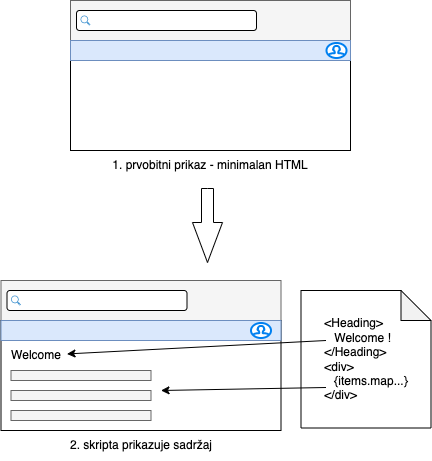
\includegraphics[width=0.6\textwidth]{docs/images/ch_4/frontend-dev-phase2.png} 
  \caption{SPA}
  \label{fig:sample}
\end{figure}

\newpage
\subsection{Hibridna okruženja}

Prethodni način generisanja korisničkog interfejsa često se naziva klijentsko renderovanje (eng. CSR - Client side rendering), dok se tradicionalni sistemi zasnivaju na serverskom renderovanju (eng. SSR - Server side rendering). Okruženja kao što su Next.js\cite{nextjsdocs}, Remix\cite{remixdocs}, SvelteKit\cite{sveltekitdocs} i druga, imaju cilj za implementaciju "najboljeg od oba sveta". Naime, omogućavaju razvoj jednostraničnih aplikacija uz podršku za serversko renderovanje, tako da otklanjaju mane u nedostatku prvobitnog prikaza HTML-a. Način njhovog rada biće prikazan u nastavku, sa izborom okruženja Next.js.

\newpage
\section{React i Next.js}
Sumirano, probleme koje treba izbeći kod tradicionalnih jednostraničnih aplikacija jesu sledeći:
\begin{enumerate}
    \item \textbf{Prvobitni HTML je minimalan.} Usled činjenice da se klijentske skripte bave prikazom korisničkog interfejsa, konkretno u React-u koristeći sistem komponenti i JSX-a \cite{reactdocscomponents}, inicijalni HTML koji se prikazuje korisniku je prazan i postoji vreme koje je potrebno dok veb pregledač izvrši skriptu.
    \item \textbf{Potrebno je dohvatiti podatke s klijenta.} Čak i nakon prikazivanja početnog korisničkog interejsa, najčešći je slučaj da je potrebno dohvatiti neke podatke preko API-a koje treba prikazati. Pošto je sva odgovornost na klijentu, ti podaci se tek mogu dohvatati u ovoj fazi, tako da postoji dodatno vreme gde neke sekcije sajta sadrže simbolične prikaze sadržaja koji se učitava\footnote{Ustanovljen naziv u frontend svetu za ove elemente jeste \textit{content loader}, postoji veliki broj biblioteka koje olakšavaju njihovo generisanje.}, dok se u pozadini vrši dohvatanje podataka.
\end{enumerate}

\subsection{React kao biblioteka i okruženje}

U ekosistemu React-a postoje nesuglasice da li React predstavlja biblioteku ili okruženje za razvoj. Argument koji ide u korist biblioteke zasniva se na činjenici da React ne poseduje striktnu strukturu direktorijuma, ne nalaže kako se vrši dohvatanje podataka, ne sadrži ugrađen sistem za rutiranje, i slično. Uzevši to u obzir zaista deluje da je React ništa više nego biblioteka za razvoj interaktivnih korisničkih interfejsa. S druge strane, vremenom su evoluiorali šabloni koji su opšteprihvaćeni kao dobre prakse, čime se može argumentovati i da je React kompletno okruženje za razvoj. Ovo je dovelo do evolucije još jednog termina koji se može sresti u onlajn zajednicama frontend inženjera, a to je metaokruženje (eng. metaframework); neretko se upravo ovom klasom softverskih sistema naziva Next.js.

\subsection{Next.js i šabloni renderovanja korisničkih interfejsa}

Imajući prethodnu diskusiju u vidu i koristeći se što opštijim terminima, može se reći da je Next.js moderno okruženje za razvoj veb aplikacija, izgrađeno nad React-om, koje podržava više šablona renderovanja korisničkih interfejsa. U trenutku pisanja ovog rada, šabloni renderovanja korisničkih interfejsa (eng. rendering patterns) čest su predmet diskusija onlajn zajednica inženjera. Najveća okruženja i biblioteke utrkuju se sa implementacijom svih šablona kako bi bili konkurentan izbor modernih frontend proizvoda. Next.js, predvođen kompanijom Vercel, definitivno je među prvima kada je u pitanju razvoj veb aplikacija. Od pomenutih šablona Next.js podržava sledeće \cite{nextjsdocs}:
\begin{itemize}
    \item \textbf{Klijentsko renderovanje - CSR.} Klasično SPA ponašanje podržano je samom činjenicom da se u osnovi nalazi React.
    \item \textbf{Serversko renderovanje - SSR.} Omogućeno je dohvatanje eksternih podataka na serveru pre renderovanja stabla React komponenti.
    \item \textbf{Generisanje statičkih sajtova - SSG\footnote{eng. Static Site Generation}.} Moguće je određene stranice u potpunosti renderovati u vremenu kompajliranja aplikacije (eng. build time), tako da gotov HTML bude spreman i pre nego što se aplikacija pokrene. Ovakve stranice po pravilu su najbrže.
    \item \textbf{Inkrementalno regenerisanje statičkih stranica - ISG\footnote{eng. Incremental Static Regeneration}.} SSG stranice jesu brze, ali mana im je što podaci mogu zastareti. Next.js omogućava periodično osvežavanje tih stranica kako bi sadržaj bio ažuran.
    \item \textbf{Strimovanje korisničkog interfejsa\footnote{eng. Streaming SSR}.} Tokom pisanja rada pojavila se React verzija 18 koja uvodi koncept serverskih komponenti (eng. server components), koje Next.js usvaja u verziji 13 i proglašava kao novi pravac. U ovom radu ovaj sistem nije razmatran, jer je u trenutku pisanja i dalje u eksperimentalnoj fazi.
\end{itemize}

\subsection{SSR i tok jednog zahteva}

SSG i ISR jesu dobar izbor prilikom generisanja sajtova koji ne menjaju svoj sadržaj često i ne bave se intenzivnom manipulacijom podataka\footnote{Dobar primer sajtova pogodnih za SSG i ISR jesu personalni blogovi.}. Ipak, sistem za kartice, koji je prikazan u ovom radu, kompleksniji je i temeljno se zasniva na dohvatanju i manipulaciji podataka sa eksternog API-a. Iz tog razloga glavni iskorišćen šablon upravo je serversko renderovanje. Na dijagramu \ref{fig:ssrdiagram} prikazan je primer toka jednog zahteva ka stranici za prikaz kartice.

\begin{figure}[h]
  \centering
  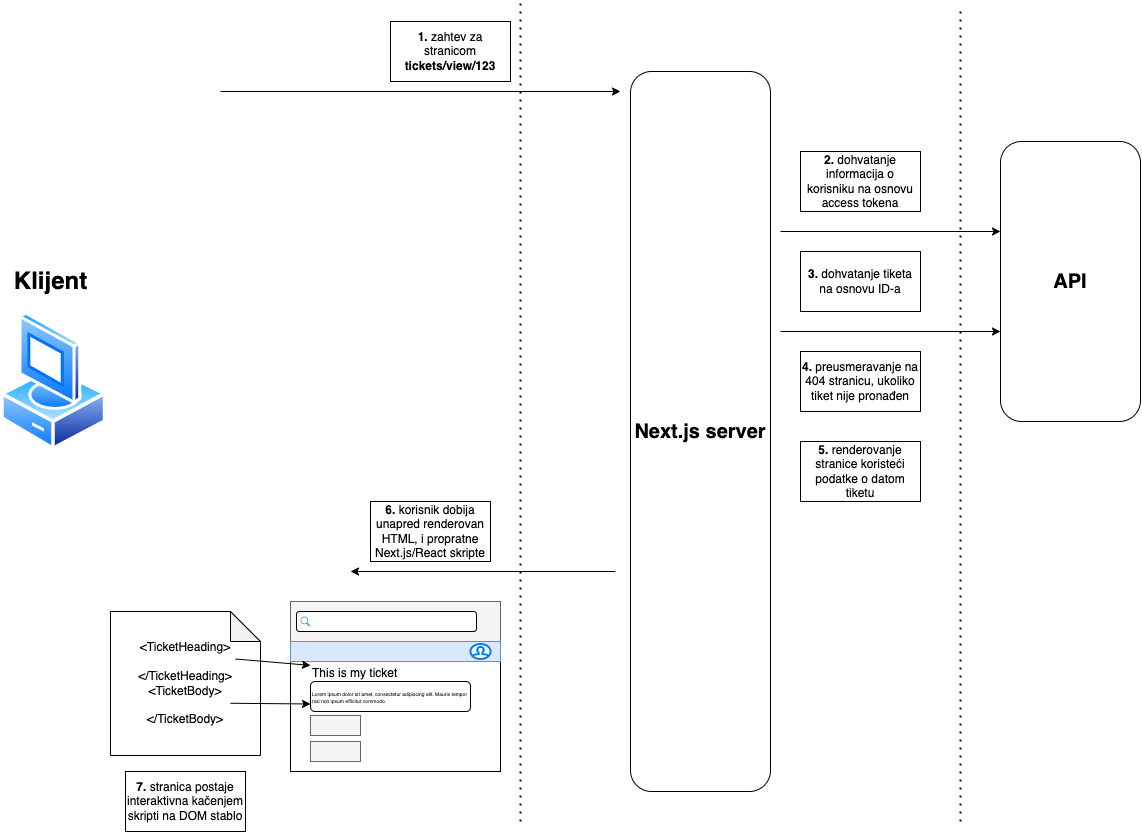
\includegraphics[width=1\textwidth]{docs/images/ch_4/nextjs_flow.png} 
  \caption{Tok jednog SSR zahteva}
  \label{fig:ssrdiagram}
\end{figure}

Proces u kom stranica postaje interaktivna, odnosno korak 7 sa dijagrama, naziva se \textbf{hidracija} \cite{reactdocscomponents}. Ovaj naziv ima smisla i može se nerformalno shvatili ako se stablo React komponenti zamisli kao sistem međusobno povezanih praznih cevi, koje se onda na vrhu prikače na izvor vode - u ovoj analogiji Javascript.

\newpage
\label{sec:datafetchingandconfiguration}
\section{Dohvatanje podataka, upravljanje stanjem, biblioteka RTK}

Kao što je pomenuto u prethodnoj sekciji, React (a tako i Next.js) prepuštaju programeru izbor načina na koji će da vrši dohvatanje podataka sa eksternih servisa. Iako to može zvučati trivijalno, dohvatanje podataka jedan je od najsloženijih zadataka modernih frontend sistema i očekivano je da React ekosistem nudi veliki broj biblioteka koji rešavaju ovaj izazov. Problemi koji se očekuju da budu rešeni od strane modernih biblioteka za dohvatanje podataka uključuju sledeće:

\begin{itemize}
    \item \textbf{Keširanje i deduplikacija.} Poželjna je mogućnost dohvatanja istih podataka u različitim delovima stabla aplikacije, a da se pritom API ne poziva svaki put, već da se podaci keširaju i iskoriste ponovo.
    \item \textbf{Deklarativnost.} Korišćenje je znatno olakšano oslobađanjem programera od pisanja proceduralne logike za dohvatanje podataka, tako što se to izvrši na deklarativan način pisanjem odgovarajuće konfiguracije.
    \item \textbf{Stanja učitavanja i grešaka.} Potrebno je imati ugrađenu podršku za stanja učitavanja (eng. loading state) i stanja grešaka (eng. error state), kako bi programer mogao da se fokusira na pisanja logike stranice u zavisnosti od tih stanja, a ne da ih manuelno prati i ažurira.
\end{itemize}

Za ovaj rad izabrana je biblioteka Redux Toolkit sa svojim podmodulom Query, koji se češće nazivaju skraćeno RTKQ \cite{rtkqdocs}. Ova biblioteka zapravo je nadogradnja na veoma poznatu biblioteku za upravljanjem stanjem\footnote{eng. state management library} Redux, koja je dugo vremena bila neizostavan deo React ekosistema. Ipak, u ovom radu ne koristi se upravljanje stanjem u pravom smislu te reči, tako da upotreba biblioteke RTKQ ostaje ograničena isključivo na dohvatanje podataka.

\subsection{Deklaracija API sloja, upravljanje keš oznakama}
U uvodnom delu ove sekcije pomenuta je deklarativnost kao jedna od tri funkcionalnosti očekivanih od moderne biblioteke za dohvatanje podataka. Deklarativnost je opšti pojam softverskog inženjerstva, i najlakši način da se opiše, neformalnim jezikom jeste "piši \textbf{šta} softver treba da uradi a ne \textbf{kako} to da uradi".

U duhu takvog načina razmišljanja, bibliteka RTKQ oslobađa programera od repetitivnog zadatka pisanja API poziva za svaki mogući entitet. RTKQ takođe pruža i elegantan mehanizam upravljanja keširanjem podataka korišćenjem koncepta keš oznaka (eng. cache tags). Naime, ako se najpre dohvati neki entitet preko određene API pristupne tačke metodom GET, a zatim ažurira metodom PATCH, prirodno je očekivati da se već dohvaćen entitet ažurira kako bi podaci prikazani korisniku  bili najsvežiji. U frontend delu aplikacije sistema STS ovakve potrebe su intenzivne prilikom operacije ažuriranja kartica.  Primer \ref{lst:rtkqconfigtickets} prikazuje kako se svi navedeni problemi rešavaju uz nekoliko jednostavnih konfiguracionih pravila koje zahteva RTKQ.

\begin{figure}[h]
\begin{lstlisting}[language=JavaScript, style=ES6, caption={Konfiguracija API poziva za dohvatanje kartice i dodavanje komentara.}, label={lst:rtkqconfigtickets}]
export const ticketsSlice = api.injectEndpoints({
  endpoints: (builder) => ({
    /* Definise se nacin na koji se dohvata kartica */
    getTicket: builder.query({
      query: ({ id, ...params }) => ({
        url: `/tickets/${id}`,
        params,
      }),
      /* Definisu se kes oznake */
      providesTags: (res) => {
        return res ? [{ type: 'getTicket', id: res.id }] : [];
      },
    }),
    addComment: builder.mutation({
      /* Definise se nacin na koji se menja kartica */
      query: ({ id, body, isInternal }) => ({
        url: `/tickets/${id}/comment/add`,
        method: 'PATCH',
        body: { body, isInternal },
      }),
      /* Definise se koje kes oznake se ponistavaju */
      invalidatesTags: ({ id }) => [{ type: 'getTicket', id }],
    }),
  }),
  overrideExisting: true,
});
\end{lstlisting}
\end{figure}

\subsection{Izazivanje dohvatanja podataka i korišćenje u komponentama}

Nakon definisanja konfiguracije u prethodnoj sekciji ostaje još pitanje načina korišćenja objekata generisanih od strane RTKQ.

Treba još jednom istaći da RTKQ nije ništa drugo nego modul sistema \verb|redux|\footnote{Tehnički, spada pod zaseban npm paket \textit{redux-toolkit}, ali u govoru se često poistovećuju jer označavaju isti ekosistem.}, tako da je očekivano da RTKQ kompletno upravljanje podacima vrši upravo posredstvom \verb|redux|-a i njegovog ugrađenog skladišta (eng. store)\footnote{Način na koji radi biblioteka \textit{redux} je kompleksan i može biti tema posebnog istraživanja, stoga je izuzeta.}. S tim u vidu, prilikom izazivanja dohvatanja podataka na serveru koristi se upravo \verb|store| objekat i RTKQ-ov poziv \verb|initiate| kako bi se dohvatanje započelo.

\begin{figure}[h]
\begin{lstlisting}[language=JavaScript, style=ES6, caption={Dohvatanje podataka o kartici na serveru.}]
export const getServerSideProps = wrapper.getServerSideProps(
  (store) => async (context) => {
    const ticketId = context.params.ticketId;
    store.dispatch(
      ticketsSlice.endpoints.getTicket.initiate({
        id: ticketId,
        ...getTicketViewQueryParams(),
      }),
    );
    // ...
    return {};
  },
);
\end{lstlisting}
\end{figure}

S druge strane, podacima se u komponentama može pristupiti odgovarajućim React udicama (eng. hooks) \cite{reactdocshooks}  koje se takođe automatski generišu. Pozivanje odgovarajućeg hook-a izaziva dohvatanje podataka klijentski, ukoliko ti podaci već ne postoje u skladištu (ukoliko već nisu dohvaćeni serverski). Hook-ovi ispoljavaju, između ostalog, stanja učitavanja, greške ili uspeha.

\begin{figure}[h]
\begin{lstlisting}[language=JavaScript, style=ES6, caption={Korišćenje RTKQ hook-ova.}]
function TicketViewPage() {
  const router = useRouter();
  const id = router.query.ticketId;

  const { isLoading, isFetching, isError } = useGetTicketQuery({
    id,
    ...getTicketViewQueryParams(),
  });
\end{lstlisting}
\end{figure}

\newpage
\subsection{Mutacije podataka}

Mutacije podataka pomenute su ukratko u \ref{sec:datafetchingandconfiguration} i prikazana je njihova konfiguracija u propratnom primeru k\^{o}da. Mutacije se skoro po pravilu koriste klijentski\footnote{Nema previše smisla izazivati mutacije podataka sa serverske strane, jer se uvek dešavaju na zahtev korisnika.}, tako da za njih RTKQ obezbeđuje hook-ove isto kao i za obično dohvatanje podataka.

\begin{figure}[h]
\begin{lstlisting}[language=JavaScript, style=ES6, caption={Korišćenje RTKQ mutacija na primeru dodavanja komentara na karticu.}]
function TicketViewPage() {
  const [addComment,
        { isLoading, isSuccess }] = useAddCommentMutation();

  const handleSubmitComment = (comment) => {
    addComment({ id: ticket.id, body: comment, isInternal });
  };
\end{lstlisting}
\end{figure}


\section{Internacionalizacija}
\label{sec:intl}

Frontend, kao deo aplikacije koji je direktno zadužen za prikaz grafičkog korisničkog interfejsa, prirodno nosi pitanja koja se odnose na način prikazivanja sadržaja neke vrste. 

Definicija internacionalizacije je veoma opšteg karaktera i na osnovu \cite{i18n} svodi se na dizajn i razvoj sadržaja proizvoda, aplikacije ili dokumenta koji omogućava lako prilagođavanje kulturi, regionu ili jeziku. U užem smislu, odnosno iz ugla frontend razvoja, razmatraju se uglavnom sadržaji sledećeg tipa:

\begin{itemize}
    \item \textbf{Tekstualni sadržaj.} Skoro svaki deo korisničkog interjsa sadrži neki tekstualni sadržaj. Iako je moguće takav sadržaj zapisati direktno u k\^{o}du (eng. hardcode), ipak je bolje imati sistem koji tekstualne sadržaje drži izdvojeno i po potrebi omogućava višejezičnost - kada korisnik promeni željeni jezik menjaju se i svi tekstualni sadržaji bez ikakve specijalne izmene u k\^{o}du.
    \item \textbf{Formati datuma i vremena.} Način zapisa datuma i vremena zavisi od regiona, tako da bi bilo dobro imati sistem takav da se te vrednosti automatski prilagođavaju korisničkom regionu.
    \item \textbf{Formati valuta.} Moguće je koristiti komponente koji automatksi konvertuju novčane iznose iz jedne valute u drugu.
\end{itemize}



U ovom radu urađena je samo prva stavka - podržani su srpski i engleksi jezik. Za potrebe čuvanja trenutnog jezika koristi se \verb|Accept-Language| HTTP zaglavlje (eng. HTTP header) u kombinaciji sa odgovarajućom vrednošću \verb|language_code| kolačića (eng. cookie) na klijentskoj strani.

U sekciji \ref{sec:tagsystem} pomenuto je kako sistem oznaka koristi internacionalizaciju za nazive i opise oznaka. Upravo podešavanje \verb|Accept-Language| zaglavlja omogućuje da API vrati podatke na odgovarajućem jeziku.

\begin{figure}[h]
\begin{lstlisting}[language=JavaScript, style=ES6, caption={Postavljanje Accept-Language zaglavlja u RTKQ prilikom API zahteva.}]
const baseQuery = fetchBaseQuery({
  baseUrl: '...',
  prepareHeaders: (headers, api) => {
    // ...
    const ctx = api?.extra?.ctx;
    const languageCode =
      (isServer()
        ? parseCookie(ctx?.req?.headers?.cookie).language_code ?? ''
        : Cookies.get('language_code')) ?? 'en';

    headers.set('Accept-Language', languageCode);
    return headers;
  },
});
\end{lstlisting}
\end{figure}

Sa druge strane, za kontrolu prikaza sadržaja na grafičkom korisničkom interfejsu koristi se kombinacija biblioteka \verb|react-intl| i \verb|formatjs| \cite{formatjsdocs}. Naime, tekstualni sadržaji, koje treba internacionalizovati na sajtu, nazivaju se \textit{poruke} (eng. messages) i definišu se odgovarajućim funkcijama u k\^{o}du, zajedno sa svojim podrazumevanim vrednostima. Primer \ref{lst:definingmessages} prikazuje definisanje nekih poruka za stranicu koja prikazuje karticu.

Pokretanjem komande \verb|npm run i18n|, definisane kao skripte u okviru fajla \verb|package.json|, vrše se \textit{ekstrakcija} i \textit{kompilacija} poruka. Ekstrakcija predstavlja proces izvlačenja svih poruka iz fajlova, koji definišu poruke na način prikazan u primeru \ref{lst:definingmessages}, u odgovarajuće JSON fajlove. Kompajliranje prevodi te fajlove u oblik prikladan korišćenju u produkciji. Delovi tih fajlova prikazani su u primeru \ref{lst:messagsjsonfiles}.

Na kraju, poruke se koriste odgovarajućin hook-ovima ili komponentama biblioteke \verb|react-intl|, kao što prikazuje primer \ref{lst:messagesusage}

\begin{figure}[h]
\begin{lstlisting}[language=JavaScript, style=ES6, caption={Definisanje poruka.}, label={lst:definingmessages}]
export const ticketViewMessages = defineMessages({
  cannotCommentOnThisTicket: {
    id: 'ticket-view.cannot-comment',
    defaultMessage: 'You cannot comment on this ticket',
  },
  publicCommentButtonText: {
    id: 'ticket-view.public-comment-button-text',
    defaultMessage: 'Public',
  },
  internalCommentButtonText: {
    id: 'ticket-view.internal-comment-button-text',
    defaultMessage: 'Internal',

\end{lstlisting}
\end{figure}

\begin{figure}[h]
\begin{lstlisting}[language=JavaScript, style=ES6, caption={JSON fajlovi sa porukama.}, label={lst:messagsjsonfiles}]
// en.json - nekompajlirana verzija
{
  "admin-link.metrics": "Metrics",
  "admin-links.home-page": "Home",
  "admin-links.tags": "Tags",
  ...

// en.json - kompajlirana verzija
{
  "admin-link.metrics": [
    {
      "type": 0,
      "value": "Metrics"
    }
  ],
  "admin-links.home-page": [
    {
      "type": 0,
      "value": "Home"
    }
  ],
  "admin-links.tags": [
    {
      "type": 0,
      "value": "Tags"
    }
  ],
\end{lstlisting}
\end{figure}

\begin{figure}[h]
\begin{lstlisting}[language=JavaScript, style=ES6, caption={Korišćenje poruka}, label={lst:messagesusage}]
const intl = useIntl();
// ...
return (<Button type="submit">
            {intl.formatMessage(formsMessages.submit)}
        </Button>)
\end{lstlisting}
\end{figure}

Treba imati u vidu da bi sofisticirani sistem internacionalizacije podržao čuvanje vrednosti u bazi podataka i njihovo eksportovanje u JSON fajlove, čime bi se omogućilo dinamičko menjanje vrednosti translacija bez ponovnog pokretanja aplikacije. To je, ipak, u ovom radu ostavljeno kao mogućnost za poboljšanje.

% ------------------------------------------------------------------------------

% ------------------------------------------------------------------------------
\chapter{Analitika}

Jedan zadatak u okviru razvoja softvera jeste napraviti sve proizvodne funkcionalnosti - kreiranje kartica, komentarisanje, promena statusa, zatvaranje, i sl. Iz ugla čistog softverskog inženjerstva moglo bi se reći da je posao završen onda kada su implementirane sve komponente sistema i njihova međusobna saradnja zarad izvršavanja poslovnih procesa.

Ovakav stav, očekivano, bio bi naivan. Problem leži u tome što ne postoji taj nivo istrage i domenskog znanja koji poslovođi može ukazati na sve potencijalne mane i moguća unapređenja sistema kao što mogu uraditi realni podaci generisani prilikom upotrebe softvera. Ovakav pristup ima za cilj da stvori ponavljajući ciklus koji se sastoji, grubo, iz sledećih koraka \cite{dataanalytics}:
\begin{enumerate}
    \item Poslovne aktivnosti se pamte u transakcionoj bazi podataka.
    \item Na osnovu tih podatka izvode se zaključci koristeći odgovarajuće tehnike i alate.
    \item Dati zaključci ukazuju na šta se treba fokusirati u razvoju proizvoda.
    \item Nove implementirane funkcionalnosti donose još podataka, koje se dalje mogu analizirati istim nizom koraka.
\end{enumerate}

\section{Skladišta podataka, ETL procesi, cron}

Niz koraka iz uvodnog dela ovog poglavlja predstavlja uopšten mentalni model na kome se zasniva proces analitike podataka\footnote{Postoji mnoštvo termina koji se koriste u današnje vreme, kao što su \textit{Data Mining, Business Intelligence} i drugi. Diskusija konkretnih pojmova je izuzeta jer ne služi svrsi ovog rada.} iz poslovnog ugla. Nešto konkretniji model, koji se više fokusira na tehnologije i metodologije, prikazan je na dijagramu \ref{fig:datadiag}.

\begin{figure}[h]
  \centering
  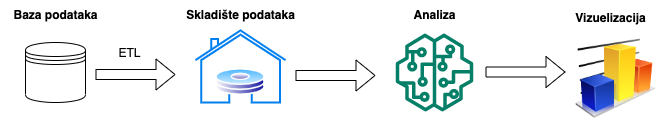
\includegraphics[width=1\textwidth]{docs/images/ch_5/datadiag.png} 
  \caption{Proces analitike.}
  \label{fig:datadiag}
\end{figure}

Za potrebe ovog rada, a iz razloga jer to nije glavni fokus, sistem analitike izveden je u uprošćenom obliku. Skladišta podataka (eng. data warehouse) predstavljaju zasebnu oblast izučavanja i u vreme pisanja rada potpadaju najviše pod oblast poznatoj kao inženjerstvo podataka (eng. data engineering). Skladište podataka posmatra se kao organizovana kolekcija podataka dobijena transformacijom izvornih podataka u oblik prikladan za izvršavanje odgovarajućih upita \cite{dataanalytics}.

Sledeće prirodno pitanje koje se nameće jeste kako i kada se date transformacije vrše. U sistemu STS ovaj zadatak potpada pod ETL (eng. Extract Transform Load) servis. Kao što i samo ime kaže sastoji se od tri koraka:
\begin{enumerate}
    \item \textbf{Extract} - izvlačenje podataka iz izvora.
    \item \textbf{Transform} - transformacija u pogodan oblik.
    \item \textbf{Load} - učitavanje u skladište podataka.
\end{enumerate}

Metrike koje mogu imati vrednost u sistemu STS jesu primarno metrike koje se odnose na karticu, kao glavni entitet, i promene koje se nad njome dešavaju. Tako se mogu razmatrati prosečno vreme rešavanja (eng. average resolution time), prosečno vreme preuzimanja (eng. average pickup time) i prosečno vreme prvog odgovora (eng. average first-response time). S tim u vidu, skladište podataka, i njegov deo koji se bavi karticama, dizajniran je tako da izvuče navedene metrike za svaku karticu\footnote{Vredi napomenuti kako je izbor šablona Event Sourcing za čuvanje kartica i niza promena prikazan u sekciji \ref{sec:eventsourcing} doprineo znatno lakšoj implementaciji ovih transformacija.}. Primer \ref{lst:ticketetlloop} prikazuje glavni deo ETL skripte. Primer \ref{lst:ticketetltransformfunction} prikazuje funkciju koja transformiše karticy, dok primer \ref{lst:ticketetlconcretefunction} prikazuje računanje jedne konkretne metrike.

Za potrebe automatizacije ovog procesa koristi se \verb|cron|, ugrađeni planer poslova (eng. job scheduler) operativnih sistema zasnovanih na Unix-u. Njegova konfiguracija je izostavljena jer nema specifičnosti u odnosnu na najosnovnije korišćenje.

\begin{figure}[h]
\begin{lstlisting}[language=python, caption={Transformacija kartice.}, label={lst:ticketetlloop}]
def main():
    # ...
    # Nalazi se poslednja obradjena kartica i njeno vreme,
    # ako postoji
    latest_processed_ticket = dest_tickets_collection.find_one(
        sort=[("timestamp", pymongo.DESCENDING)]
    )
    latest_timestamp = \
        latest_processed_ticket["timestamp"] \
        if latest_processed_ticket else None

    # Uzimaju se sve neobradjene kartice
    query = {}
    if latest_timestamp:
        query["timestamp"] = {"$gte": latest_timestamp}

    unprocessed_tickets_cursor = src_tickets_collection.find(query)

    # Transformisu se sve neobradjene kartice
    new_tickets = []
    for ticket in unprocessed_tickets_cursor:
        
        transformed_ticket = transform_data(ticket)
        new_tickets.append(transformed_ticket)

    # Ubacuju se u skladiste
    if new_tickets:
        dest_tickets_collection.insert_many(new_tickets)
\end{lstlisting}
\end{figure}

\begin{figure}[h]
\begin{lstlisting}[language=python, caption={Funkcija koja transformiše podatke.}, label={lst:ticketetltransformfunction}]
def transform_data(ticket):
    created_at = ticket.get('createdAt')
    resolution_time, resolution_timestamp = \
        calculate_resolution_time(ticket)
    pickup_time, pickup_timestamp = \
        calculate_pickup_time(ticket)
    first_response_time, first_response_timestamp \
        = calculate_first_response_time(ticket)
    status = ticket.get('status')

    return {"_id": ticket.get('_id'),
            "timestamp": created_at,
            "resolution_time": resolution_time,
            "resolved_at": resolution_timestamp,
            "pickup_time": pickup_time,
            "picked_up_at": pickup_timestamp,
            "first_response_time": first_response_time,
            "first_responded_at": first_response_timestamp,
            "status": status}
\end{lstlisting}
\end{figure}

\begin{figure}[h]
\begin{lstlisting}[language=python, caption={Računanje konkretne metrike.}, label={lst:ticketetlconcretefunction}]
def calculate_resolution_time(ticket):
    created_at = ticket.get('createdAt')

    history = ticket.get('history')
    resolution_time_items = list(filter( \ 
        lambda item: item.get('type') == 'STATUS_CHANGED' \
        and item.get('payload').get('status') == 'RESOLVED', \
        history))

    resolved_time = resolution_time_items[-1].get(
        'timestamp') if resolution_time_items else None

    resolution_time = \
        (resolved_time - created_at).total_seconds() / 60 \
        if resolved_time else None

    return resolution_time, resolved_time
\end{lstlisting}
\end{figure}



\newpage
\section{Prikaz metrika, biblioteka streamlit}

Nakon uspešnog punjenja skladišta podataka postoje dva pravca, kojima tok podataka može dalje ići. Pritom treba imati u vidu da ta dva pravca nisu međusobno isključiva.
\begin{itemize}
    \item Podaci iz skladišta mogu se koristiti za naprednu analizu statističkim metodama ili metodama mašinskog učenja.
    \item Podaci se mogu vizuelizovati određenim kontrolnim tablama (eng. dashboards) zarad brzog dobijanja slike o podacima.
\end{itemize}

Kao što je već napomenuto, napredne analize podataka ne spadaju u područje ovog rada, ali jednostavna vizuelizacija podataka izvučenih u prethodnom poglavlju implementirana je \textit{python} bibliotekom \textit{streamlit} \cite{streamlitdocs}.

Ova biblioteka omogućava jednostavno kreiranje interaktivnih kontrolnih tabli za prikaz podataka. Glavna prednost je u tome što sadrži veliki broj predefinisanih elemenata korisničkog interfejsa (grafikoni, histograni, prikaz vremena, elementi za odabir opsega datuma, i slično) što omogućava programeru da se fokusira na poslovne vrednosti umesto na tehnikalije izgradnje takvih elemenata. 

Skripta za prikaz kontrolne table je jednostavna i može se videti u fajlu \verb|services/analytics/app.py|. Sastoji se od dohvatanja informacija o karticama za izabran vremenski okvir i prikaz prosečnih vrednosti statistika iz prethodnog poglavlja. Slika \ref{fig:stsmetrics} prikazuje izgleda korisničkog interfejsa ove kontrolne table.

\begin{figure}[h]
  \centering
  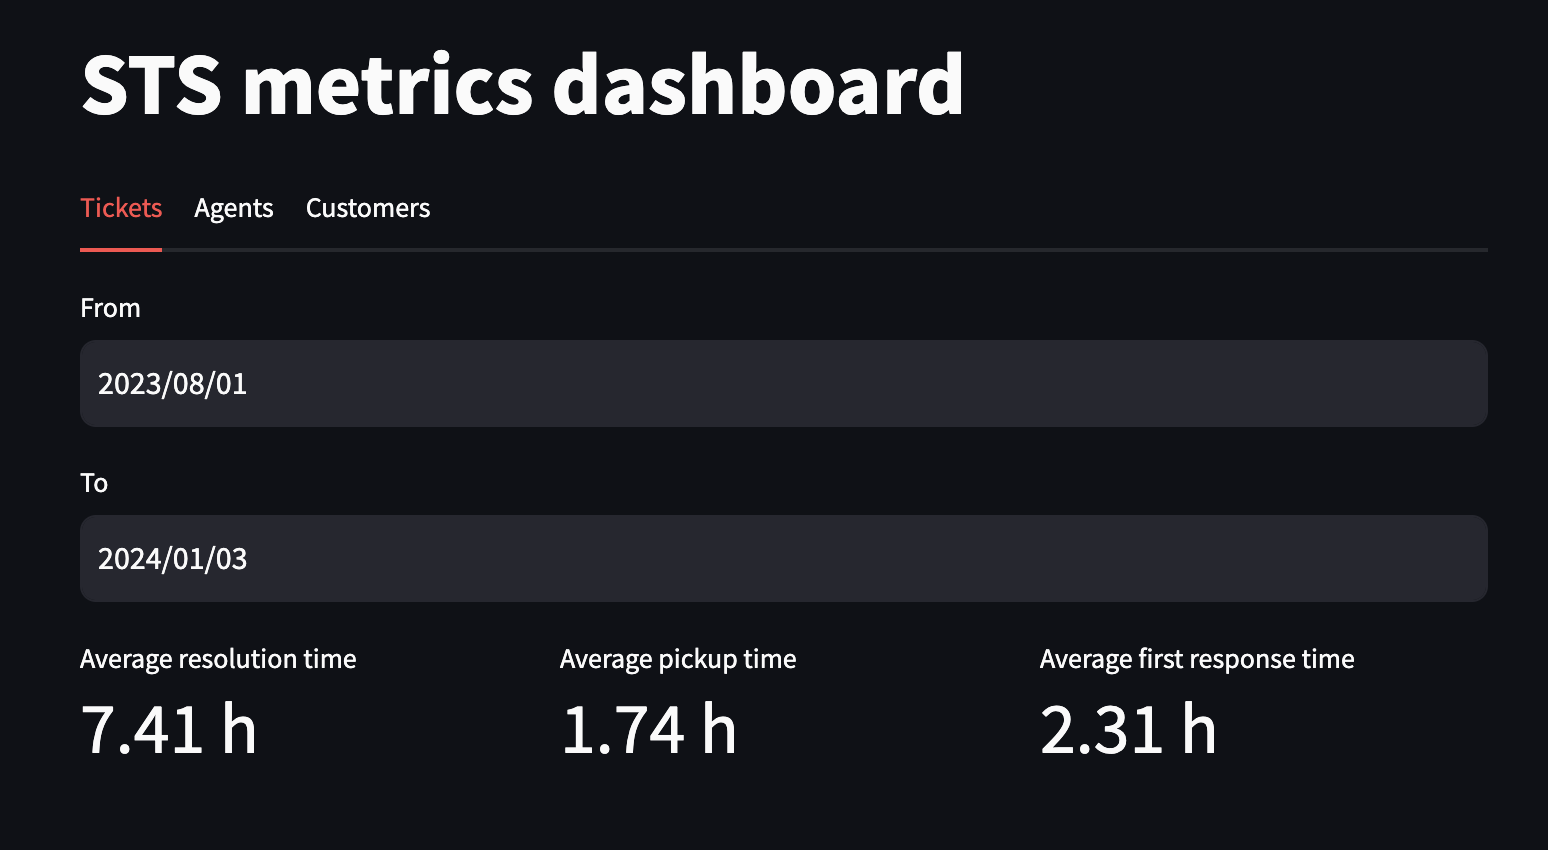
\includegraphics[width=1\textwidth]{docs/images/ch_5/stsmetrics.png} 
  \caption{Kontrolna tabla STS analitike.}
  \label{fig:stsmetrics}
\end{figure}

% ------------------------------------------------------------------------------

% ------------------------------------------------------------------------------
\chapter{DevOps}

Pojam DevOps (nastao od engleske sintagme \textit{Development Operations} - u bukvalnom prevodu \textit{razvojne operacije}) predstavlja relativno mladu granu softverskog inženjerstva. U svojoj najužoj definiciji, prema \cite{zdevopsarticle}, kaže se da DevOps opisuje usvajanje iterativnog razvoja softvera, automatizaciju i programabilne infrastrukture za otpremanje\footnote{eng. deployment} i održavanje softverskog sistema.

U nekim krugovima poistovećuje se sa ulogom sistemskih administratora dok drugi tvrde da je to potpuno zasebna profesija. Obe strane moraju se složiti da sa masovnim razvojem različitih tehnologija, okruženja i platformi nastaju novi problemi koji ne potpadaju pod tradicionalni pojam softverskog inženjerstva koji uglavnom obuhvata razvoj domenskih funkcionalnosti. Naime, ukoliko je zadatak \textit{"implementirati dugme na stranici za prikaz kartice kojim se zatvara kartica"} potpuno je jasno da se tim zadatkom neće baviti DevOps inženjer, dok bi na primer zadatak \textit{implementirati sistem za periodično pravljenje i čuvanje rezervnih kopija baze podataka} upravo zapao tom inženjeru.

Interesantno opažanje primećeno u \cite{devopshandbook} je da u mnogim kompanijama postoji neprekidna kontrateža između odeljenja za razvoj i odeljenja za razvojne operacije, uprkos činjenici da je kranji cilj isti. Na primer, inženjeru kome je zadatak da implementira jedan mali server za nekoliko API pristupnih tačaka od nule biće lakše da taj server pokrene direktno na produkcionoj mašini i neretko će zahtevati da se "napravi izuzetak" usled skromne veličine projekta. DevOps inženjer bi skoro sigurno insistirao na tome da se čak i za najmanji takav server napravi odgovarajuća infrastruktura, recimo kroz Docker. Lako je zapitati se zašto se uopšte dovodi u pitanje vrednost poštovanja principa razvojnih operacija i zašto bi programer iz hipotetičkog scenarija ikada zahtevao da se napravi izuzetak. Odgovori na ova pitanja zalaze u poslovne aspekte softverskog inženjerstva gde je uvek pitanje toga ko donosi veću vrednost. Ovaj rad se uzdržava od dalje diskusije na tu temu jer je fokus primarno tehnički, ali vredi napomenuti da su istorijat DevOps-a i razni poslovni aspekti ove grane odlično obrađeni u \cite{devopshandbook}.


\section{Kontejneri, sistem Docker}

Istorija nastajanja Docker-a, i kontejnerizacije uopšte, interesantna je tema sama za sebe i u \cite{dockerdeepdive} izložena ukratko na sledeći način:
\begin{enumerate}
    \item \textbf{Korišćenje zasebnih servera za svaku aplikaciju.} U početku je bilo komplikovano, pa čak i nemoguće pokrenuti više zasebnih servera na istoj mašini, tako da bi kompanije često išle u pravcu kupovanja ili iznajmljivanja zasebnih fizičkih servera za svaki aplikativni server.
    \item \textbf{Virtuelne mašine.} Koncept koji je značajno olakšao stvari bile su virtuelne mašine. Dozvoljavale su pokretanje proizvoljnog broja istinski odvojenih okruženja na jednoj fizičkoj mašini. Mana ovakvog pristupa jeste da virtuelna mašina zahteva kompletan operativni sistem, a samim tim i dosta resursa u vidu RAM-a i procesorskog vremena.
    \item \textbf{Kontejneri.} Kao rešenje koje ima za cilj da uzme najbolje od oba sveta nastaju kontejneri (eng. containters). Za razliku od virtuelnih mašina, svaki pokrenut kontejner koristi operativni sistem računara na kome se pokreće, a ipak održava nivo potpune izolovanosti.
\end{enumerate}

Docker je jedno od rešenja za rad sa kontejnerima, i izabrano je za potrebe ovog rada usled svoje popularnosti i rasprostranjenosti. Za mnoge programere, čija je primarna delatnost razvoj poslovnih funckionalnosti, Docker predstavlja crnu kutiju. Pojmovi kao što su \textit{docker engine}, \textit{slike (eng. images)} i \textit{orkestracija} stvaraju konfuziju ako se od početka ne posveti pažnja njihovom razumevanju, stoga se naredne sekcije koristite analogijama sa nekim konceptima koji su poznati svim pogramerima.

\subsection{Docker slike}

Na početku poglavlja pomenuto je kako je jedan od zadataka DevOps-a, između ostalog, uspostavljanje programabilnog infrastruktura za otpremanje i održavanje softverskog sistema. Način pravljenja docker slika upravo se zasniva na programabilnosti. 

Naime, docker slike treba shvatiti upravo po inspiraciji zbog koje se koriste - postoji potreba za izolovanim okruženjem jako specifične namene. Pomenuto je da virtuelne mašine nose sa sobom previše stvari za kojim ne postoji potreba, najpre ceo operativni sistem i svi njegove module. Definicijom adekvatne docker slike izbegava se korišćenje bespotrebnih resursa. 

Dakle, prilikom definisanja slike za pokretanje bekend servera sistema STS u režimu za razvoj\footnote{O produkcionoj postavci biće reči kasnije.}, pristupa se sledećim prirodnim rezonovanjem:

\begin{enumerate}
    \item Potreban je Node.js
    \item Potreban je CLI za okruženje \verb|@nestjs|
    \item Potrebno je instalirati sve pakete deklarisane u fajlu \verb|package.json|
    \item Potrebno je prekopirati izvorni k\^{o}d
    \item Potrebno je pokrenuti razvojni server
\end{enumerate}

Jezik kojim se prave docker slike upravo je pravljen da što bliže oslika prirodni jezik opisivanja sistema, i prikazan je na \ref{lst:dockerimgbackendexample}.

\begin{figure}[h]
\begin{lstlisting}[language=docker, caption={Slika za bekend server}, label={lst:dockerimgbackendexample}]
FROM node:18-alpine3.16

# Basic setup
WORKDIR /app
ENV NODE_ENV=development

# Install nestjs cli
RUN npm i -g @nestjs/cli@9.3.0

# Install dependencies first to utilize build cache
COPY package*.json ./
RUN npm install

# Copy the sourcecode
COPY . .

# Start the development server
CMD ["npm", "run", "start:dev"]
\end{lstlisting}
\end{figure}

\subsection{Docker kontejneri}

U analogiji između razvoja slika i kontejnera sa običnim razvojem aplikacija moglo bi se reći da slika odgovara programu, a kontejner odgovara procesu. Na taj način gore definisana docker slika sama po sebi ne radi ništa ukoliko se ne pokrene u vidu kontejnera. 

Nastavljajući analogiju, sliku se prvo mora izgraditi (eng. build) što bi odgovaralo procesu kompilacije. Ovu kompilaciju je bolje shvatiti ne kao prevod na mašinski jezik, već kao prevod u međureprezentaciju, koju je u stanju da izvršava docker engine. Docker CLI komandom, na primeru \ref{lst:buildinglocal}, gradi se slika sa odgovarajućom oznakom (eng. tag).

\newpage
\begin{lstlisting}[caption={Izgradnja slike}, label={lst:buildinglocal}]
docker build -f
    services/api-main/docker/Dockerfile.development 
    -t sts-api-local 
    ./services/api-main 
\end{lstlisting}

Nakon izgradnje moguće je pokrenuti datu sliku u vidu kontejnera, sa nekoliko dodatnih konfiguracija koje se sastoje od sledećeg:
\begin{itemize}
    \item \textbf{Vezivanje portova.} Opcijom \verb|-p| navodi se koji port kontejnera se vezuje za koji port domaćinskog operativnog sistema (eng. host OS). Ovo omogućava da aplikacija unutar kontejnera bude agnostična od zauzetosti portova.
    \item \textbf{Povezivanje sa fajl sistemom.} U lokalnom razvojnom okruženju potreban je izvorni k\^{o}d aplikacije, koji se može uvesti korišćenjem koncepta \textit{docker volume}-a. Oni predstavljaju apstrakciju medijskih uređaja, ali u ovom slučaju koriste se za povezivanje određenih direktorijuma unutar kontejnera sa hostom\footnote{Ovo se ostvaruje tehnologijom rsync. Detalji su izostavljeni, ali vredi napomenuti jer se u praksi često koristi izraz rsync kao glagol. Neretko se može čuti izraz da su dva foldera "rsync-ovana".}.
\end{itemize}

Primer komande za pokretanje prikazan je u \ref{lst:dockerrunninglocal}.

\begin{lstlisting}[caption={Pokretanje kontejnera}, label={lst:dockerrunninglocal}]
docker run 
    sts-api-local 
    -v ./services/api-main:/app 
    -p 3000:3000
\end{lstlisting}

U skladu sa analogijom, kompajlirani program je sada pokrenut i sada predstavlja proces.

\subsection{Orkestracija putem modula docker-compose}

Proces prikazan u prethodne dve sekcije izgleda previše repetitivno i, još bitnije, deluje da se može automatizovati. Prikazani način razvoja doveo bi do konstantnog ponavljanja sledećih koraka:
\begin{enumerate}
    \item Izgradi sve slike komandama \verb|docker build|.
    \item Pokreni sve kontejnere komandama \verb|docker run|.
\end{enumerate}

Pritom se uvek mora voditi računa da li se odgovarajući portovi dobro vezuju, da li se vezani odgovarajući fajlovi i slično. Dijagram ovog procesa prikazan je na slici \ref{fig:dockermanual}. Čitav ovaj proces upravljanja stanjima kontejnera, njihovim pokretanjem i obaranjem, portovima i vezivanjem sa fajl sistemom podvodi se pod jedan sveobuhvatni pojam \textit{orkestracije}.

\begin{figure}[h]
  \centering
  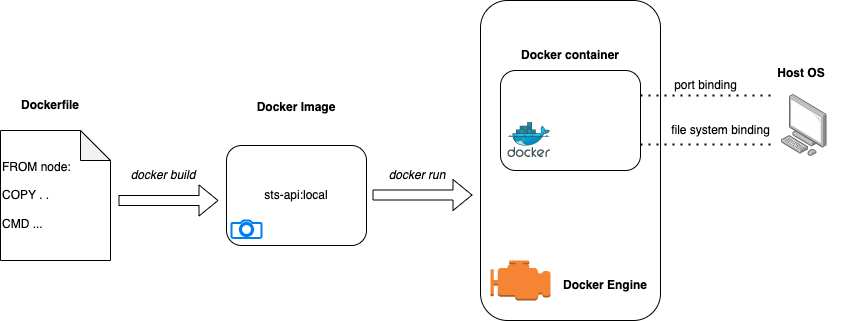
\includegraphics[width=1\textwidth]{docs/images/ch_6/dockermanual.png} 
  \caption{Proces pokretanja kontejnera.}
  \label{fig:dockermanual}
\end{figure}

Postoje vrlo sofisticirani softverski sistemi za orkestraciju kontejnera, od kojih se neki pokreću primarno u oblaku\footnote{Primer takvog sistema je AWS ECS.}. Sistem STS nije dizajniran za cloud okruženja već za varijantu samostalnog hostovanja (eng. self-hosting)\footnote{Jedna zanimljivost je da tokom pisanja ovog rada postoji veliki raskol u onlajn zajednicama programera: da li je bolje koristiti cloud rešenja ili samostalno hostovanje. Slična rasprava vodi se oko promovisanja monolitnih okruženja kao superiornih u odnosu na mikroservise, što nekima deluje kao vraćanje u prošlost.}. Zbog toga orkestrator docker-compose zadovoljava sve zahteve.

Skoro svi orkestratori zasnivaju se na konfiguraciji umesto na eksplicitnom programiranju ponašanja kontejnera (kao što je prvobitno urađeno koristeći \verb|bash| skripte iz prethodnih sekcija). U slučaju docker-compose-a to se postiže pisanjem YAML fajlova. Konfiguracija u ovom fajlovima navodi koje sve servise sistem sadrži, koju sliku koriste ili na koji način se izgrađuju, konfiguracije portova i vezivanja fajl sistema, promenljive okruženja i slično. Primer konfigurisanja bekend i frontend servisa za lokalno okruženje dat je u \ref{lst:dockercomposelocal}.

Nakon ovakvog konfigurisanja čitavog sistema, upravljanje kompletnim okruženjem poprilično je jednostavno i može se postići sa nekoliko jednostavnih komandi prikazanih u \ref{lst:dockerlocalcommands}.

\begin{figure}[h]
\begin{lstlisting}[language=docker-compose, caption={docker-compose konfiguracija nekih razvojnih servisa.}, label={lst:dockercomposelocal}]
services:
  api_main:
    container_name: api-main-local
    build:
      context: ./services/api-main
      dockerfile: ./docker/Dockerfile.development
    environment:
      MAIN_DB_USERNAME: ${MAIN_DB_USERNAME}
      MAIN_DB_PWD: ${MAIN_DB_PWD}
      JWT_SECRET: ${JWT_SECRET}
      FIREBASE_KEY_PATH: "/app/certificates/sts-firebase-key.json"
    ports:
      - "3001:3000"
    volumes:
      - "./services/api-main:/app"
    extra_hosts:
      - "host.docker.internal:host-gateway"

  ssr:
    container_name: ssr-local
    build:
      context: ./services/ssr
      dockerfile: ./docker/Dockerfile.development
    ports:
      - "3003:3000"
    environment:
      NODE_ENV: "development"
      NODE_TLS_REJECT_UNAUTHORIZED: "0"
    volumes:
      - "./services/ssr:/app/"
    extra_hosts:
      - "host.docker.internal:host-gateway"
\end{lstlisting}
\end{figure}

\newpage
\begin{lstlisting}[caption={docker-compose komande.}, label={lst:dockerlocalcommands}]
# Pokretanje svih servisa
docker-compose up -d 

# Obaranje svih servisa
docker-compose down
\end{lstlisting}

Vredi napomenuti da docker-compose podržava i kompleksnije operacije kao što su skaliranje kontejnera\footnote{Uz propratne module kao što su docker-swarm.}, koje su van okvira ovog rada. Ta činjenica ima za cilj da obeshrabri popularno mišljenje da se za bilo kakav ozbiljan rad sa kontejnerima mora odmah pribegavati naprednim sistemima kao što su \textit{AWS ECS} ili \textit{kubernetes}. Naravno da ti sistemi imaju svoju ulogu i veoma su moćni, ali njihovo preuranjeno korišćenje može doneti više štete nego koristi razvoju.


\section{Reverzni proksi nginx}

Uspostavljanjem docker-a kao sistema za pokretanje aplikacije rešen je jedan problem - izolacija okruženja. U ovom trenutku postoji pet servisa pokrenutih kroz različite kontejnere i povezane na različite portove\footnote{Servisi su: baza podataka, Nest.js server, Next.js server, ETL i streamlit.}. Sledeće pitanje koje se prirodno nameće jeste kako korisnik pristupa veb sajtu i kako servisi komuniciraju jedni između drugih. Uzevši u obzir da se svi servisi pokreću na različitim portovima, bilo bi neodrživo da svaka komponenta sistema mora da zna na kojim portovima su ostale, a potpuno apsurdno da korisnik sajta mora da zna na kom portu je hostovan glavni vebsajt (frontend).

Očigledna je potreba za pristupnom tačkom celog sistema za spoljašnji svet - jednom rečju potreban je \textbf{veb server}. Pri početku pogavlja \ref{sec:backend} izričito je napomenuta razlika između veb servera i aplikativnog servera. Pod aplikativnim serverom podrazumeva se HTTP server u odgovarajućem veb okruženju (u ovom slučaju Next.js ili Nest.js) koji služi za obradu zahteva ili (u slučaju serverskog renderovanja) generisanje HTML-a. Ovi serveri treba da se bave isključivo svojim ulogama i da se ne brinu o stvarima kao što su provera SSL sertifikata, serviranje statičkih fajlova i slično. Navedeni zadaci, naravno uz još mnoge, potpadaju pod ulogu veb servera.

Tok korisničkog zahteva može se uprošćeno shvatiti na sledeći način, kao što je prikazano u \cite{webvsappserver}:
\begin{enumerate}
    \item Korisnik pokuša da pristupi određenom resursu putem URL-a.
    \item Zahtev prvo stiže do veb servera\footnote{Ukoliko se dodatno koristi mreža za dostavljanje sadržaja (eng. Content Delivery Network - CDN), recimo Cloudflare, onda bi zahtev tehnički prvo prošao kroz nju, ali svakako veb server treba da bude agnostičan od toga.}. Ukoliko se koristi HTTPS, veb server vrši proveru sertifikata i bezbednosti konekcije.
    \item U zavisnosti od URL-a, veb server odlučuje da li može sam da odgovori ili ne. Ukoliko može, na primer ako je zahtev za statičkim sadržajem kao što su slike, veb server odgovara i komunikacija se završava.
    \item U suprotnom veb server delegira posao odgovarajućem aplikativnom serveru.
\end{enumerate}

$nginx$ \cite{nginxdocs} omogućava sve od navedenog. Kada se koristi za delegiranje zadataka aplikativnim serverima, onda se kaže da zauzima ulogu obrnutog ili reverznog proksija (eng. reverse proxy). Razlog takvog imenovanja jeste upravo u smeru prosleđivanja zahteva - klasičan proksi prosleđuje zahteve eksternim servisima, dok reverzni proksi prosleđuje zahteve "sam na sebe". 

Dijagram \ref{fig:dockerandnginxfinal} prikazuje nacrt celog sistema.


\begin{figure}[h, width=0.5]
  \centering
  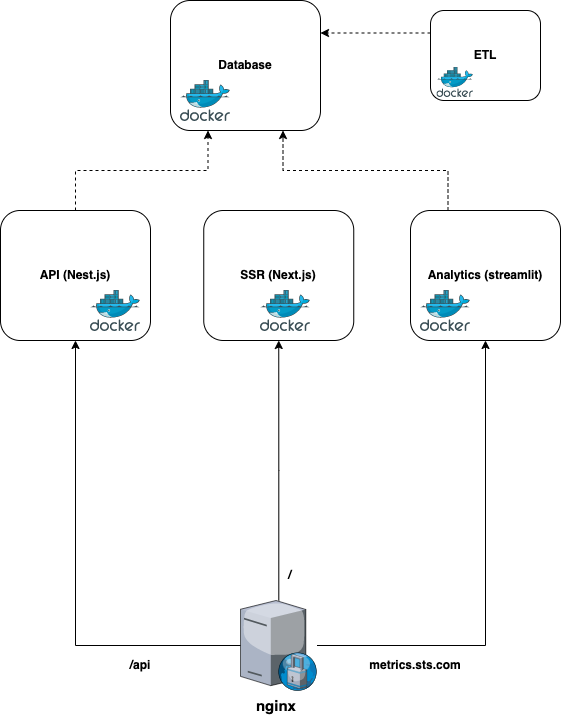
\includegraphics[width=1\textwidth]{docs/images/ch_6/dockernadnginxfinal.png} 
  \caption{Nacrt sistema.}
  \label{fig:dockerandnginxfinal}
\end{figure}


\newpage
\section{Produkciono okruženje, višefazna izgradnja slika, DockerHub}

Za kraj istaknute se male razlike između konfiguracije lokalnog okruženja, prikazanog u prethodnim sekcijama, i produkcionog, od čega je najveća razlika u docker slikama. Naime, u produkciji nema potrebe za otpremanjem izvornog k\^{o}da aplikacija, kao što se to radi u lokalnom okruženju\footnote{U lokalnom okruženju potreban je izvorni k\^{o}d kako bi promene u k\^{o}du bile odmah vidljive, bez ikakve kompilacije ili izgradnje.}, već se u docker sliku mogu kopirati samo fajlovi neophodni za pokretanje.


\subsection{Višefazna izgradnja}
Na primer, u slučaju Nest.js API-a dovoljno je imati samo nekoliko fajlova i foldera: 
\begin{itemize}
    \item \verb|node_modules| folder koji sadrži instalirane Node.js pakete.
    \item \verb|dist| folder koji sadrži kompajliran produkcioni k\^{o}d.
    \item \verb|package.json| fajl za pokretanje skripti.
\end{itemize}

Izgradnja docker slika koje sadrže samo potrebne fajlove, i odbacuju sve što nije potrebno usput, postiže se korišćenjem višefaznih izgradnji (eng. multiphase build). Dockerfile se može organizovati u više faza, gde se iz svake faze kopiraju isključivo fajlovi koji su potrebni na samom kraju. Ovakav način izgradnje slika prikazan je u primeru \ref{lst:mfbuild}.

\begin{figure}[h]
\begin{lstlisting}[language=docker, caption={Višefazna izgradnja slike za API servis.}, label={lst:mfbuild}]
# Install deps
FROM node:18-alpine3.16 as deps
WORKDIR /app
COPY ./package.json ./
COPY ./package-lock.json ./
RUN npm ci

# Build
FROM node:18-alpine3.16 as builder
WORKDIR /app
COPY --from=deps /app/node_modules ./node_modules
COPY . .
RUN npm run build

# Run
FROM node:18-alpine3.16 as runner
WORKDIR /app
ENV NODE_ENV production
COPY --from=deps /app/node_modules ./node_modules
COPY --from=builder /app/package.json ./package.json
COPY --from=builder /app/dist ./dist
EXPOSE 3000
ENV PORT 3000
CMD ["node", "dist/main"]
\end{lstlisting}
\end{figure}

\newpage
\subsection{DockerHub}

Kao dodatno olakšanje za pokretanje produkcione varijante sistema STS, slike se mogu otpremiti na DockerHub, koji predstavlja onlajn servis za pronalaženje i deljenje docker slika \cite{dockerhubdocs}. Besplatan plan koji nudi DockerHub, u trenutku pisanja ovog rada, omogućava hostovanje neograničeno mnogo javnih slika, što je više nego dovoljno za potrebe sistema STS. 

S tim u vidu napravljene su produkcione skripte, koje se nalaze u folderu \verb|bin| u izvornom k\^{o}du i bave se izgradnjom i otpremanjem produkcionih slika. Primer ovih komandi prikazan je u \ref{lst:prodscriptsexample}.

\begin{lstlisting}[caption={docker-compose komande.}, label={lst:prodscriptsexample}]
# Komanda za izgradnju API slike (fajl sts-build)
docker build -f 
    ./services/api-main/docker/Dockerfile.production 
    -t aleksakojadinovic/sts:api-latest 
    ./services/api-main

# Komanda za otpremanje slike (fajl sts-push)
docker push aleksakojadinovic/sts:api-latest

\end{lstlisting}

Produkciona docker-compose konfiguracija sada ne mora uopšte zavisiti od postojanja Dockerfile-ova, već može direktno pokretati slike sa DockerHub-a. Na taj način postignuto je da na konačnom fizičkom\footnote{Fizička karakteristika servera je naglašena jer se podrazumeva prava instanca servera gde će se pokretati docker. Ipak pojam fizičkog servera i ovde treba uzeti sa rezervom jer su u oblaku i takvi serveri virtuelni samo na višem nivou. Svakako iz ugla korisnika smatraju se za fizičke servere.} serveru, na kom se pokreće sistem, nije potrebno niti imati izvorni k\^{o}d niti klonirati git repozitorijum izvornog k\^{o}da - docker-compose konfiguracija može se držati u zasebnom repozitorijumu. Ipak je sve obuhvaćeno u jednom repozitorijumu kako bi služio kao centralni izvor svega pokrivenog u radu.

% ------------------------------------------------------------------------------

% ------------------------------------------------------------------------------
\chapter{Zaključak}
% ------------------------------------------------------------------------------

Dostupne tehnologije za razvoj veb aplikacija su mnogobrojne i trendovi ukazuju na to da će ih biti sve više. Tehnološki stekovi (eng. tech stack) mogu se neformalno svrstati u dve grupe. Prva bi se sastojala od tradicionalnih ekosistema poput onih vezanih za jezik PHP\footnote{Uz koji često ide MySQL baza podataka, sa podrškom okruženja kao što je CodeIgniter, Symfony ili Laravel.} ili Javu\footnote{Npr. okruženje Spring Boot.}, dok bi se u drugu mogli svrstati moderne Javascript biblioteke, od kojih su neke prikazane. Nije retka pojava izjednačavanje tradicionalnih okruženja sa kvalitetom i stabilnošću, i stav da se jedino u njima može pisati ozbiljan softver. Isto tako postoji i pogrešno verovanje u suprotnom smeru - novi Javascript ekosistemi označavaju se kao infantilni uprkos dugogodišnjem postojanju.

Cilj ovog rada je višestruk. Sa jedne strane služi da potvrdi činjenicu da je dobra infrastruktura i dizajn softvera agnostičan od konkretnih tehnologija. Druga svrha jeste prikaz kompletnog procesa razvoja složenog softverskog sistema u modernim tehnologijama, a pritom ne pribegavajući brzim rešenjima koja okruženja nude već prateći ustanovljene principe.

Već u prvom poglavlju dat je primer dizajna nerelacione baze podataka putem ER modela, koji se često vezuje čvrsto za relacione baze. Pritom je iskorišćen šablon Event Sourcing zarad povećanja fleksibilnosti kartica. Kasnije, uvođenjem okruženja NestJS i jezika \verb|typescript|, a uz podršku paketa \verb|mongoose|, implementacija principima domenskog dizajna omogućila je maksimalnu izolovanost slojeva. Razlika između osnovnog entiteta kroz tri sloja - infrastrukturni, domenski i API - demonstrira istinsku izolovanost komponenti i omogućava razmišljanje o izdvajanju u zasebne pakete, ili čak mikroservise.

Frontend svet je u trenutku pisanja raznovrsan i podeljen. Pojava da velika kompanija kao što je Vercel predvodi okruženje otvorenog k\^{o}da (Next.js) dovodi do toga da marketing i popularnost utiče direktno na šablone razvoja softvera\footnote{Na primer, moguće je direktno se povezati na bazu podataka u Next.js-u i vršiti upite na bazi zahteva. Jasno je da ovde sprega između frontend dela aplikacije i baze podataka ogromna, a ipak se ovakav pristup reklamira kao poželjan u određenim Next.js kursevima.}. Ovaj rad je iz tog ugla stremio da uzme najbolje iz oba sveta - iskorišćen je pun potencijal serverskog renderovanja Next.js-a, a uz podršku stabilnih ekosistemskih paketa poput redux-a.

Poglavlje o DevOps-u prikazuje moć Docker-a kao univerzalnog alata za izolaciju okruženja i otpremanje softvera. Za ogromne sisteme cloud rešenja koja nude veliki provajderi poput Amazona ili Google-a mogu biti dobar izbor, ali treba imati u vidu da kombinacija alata kao što su Docker i nginx mogu zadovoljiti većinu potreba.

Analitika može biti tema za zasebno istraživanje, ali je uspešno uspostavljena platforma za njen dalji razvoj.

Naravno, sistem STS, čija je implementacija dostupna javno na adresi \\\href{https://github.com/aleksakojadinovic/master_rad}{https://github.com/aleksakojadinovic/master\_rad}, u obliku prikazanom u ovom radu ima očiglednih nedostataka. Najočigledniji nedostatak jesu testovi - jedinični testovi (eng. unit tests) bili bi krucijalan deo za garanciju kvaliteta softvera i deo procesa otpremanja. Zamerka se može ukazati i na infrastruktuni sloj bekenda i njegov strogi izbor pohlepnog učitavanja - neki sistemi omogućavaju odabir da li je učitavanje lenjo ili pohlepno na nivou entiteta. Nedostatak tipiziranja u frontendu, odnosno korišćenje čistog jezika \verb|javascript|, stvar je izbora zarad izbegavanja kompleksnosti. Iz ugla osiguravanja podataka, automatske skripte za generisanje rezervnih kopija baze podataka bile bi neizostavan deo ozbiljnog softverskog sistema u produkciji, što se može postići kako manuelno tako i korišćenjem baza podataka u oblaku. Analitički servis, kao što je pomenuto, jeste minimalan i služi isključivo za demonstraciju takvih mogućnosti.

Sve u svemu, trenutna implementacija sistema STS čini solidnu osnovnu za dalji razvoj. Izolovanost komponenti omogućava i laku podelu poslova po timovima, kako bi svaki tim mogao da se fokusira na unapređenje pojedinačnih modula. Programski k\^{o}d u repozitorijumu može poslužiti i kao šablon za buduće projekte (eng. boilerplate) sa izborom istih tehnologija.
% ------------------------------------------------------------------------------
% Literatura
% ------------------------------------------------------------------------------
\literatura

% ==============================================================================
% Završni deo teze i prilozi
\backmatter
% ==============================================================================

% ------------------------------------------------------------------------------
% Biografija kandidata
\begin{biografija}
\textbf{Aleksa Kojadinović} rođen je 1998. godine u Užicu, gde završava osnovno i srednje obrazovanje. Nakon toga upisuje informatički smer Matematičkog fakulteta u Beogradu. Osnovne studije završava 2021. godine, a odmah nakon diplomiranja upisuje master studije na istom smeru. U međuvremenu zapošljava se u kompaniji FishingBooker kao Frontend softverski inženjer, specijalizovan za Javascript tehnologije.
\end{biografija}
% ------------------------------------------------------------------------------

\end{document} 
